\documentclass[twoside]{book}

% Packages required by doxygen
\usepackage{fixltx2e}
\usepackage{calc}
\usepackage{doxygen}
\usepackage[export]{adjustbox} % also loads graphicx
\usepackage{graphicx}
\usepackage[utf8]{inputenc}
\usepackage{makeidx}
\usepackage{multicol}
\usepackage{multirow}
\PassOptionsToPackage{warn}{textcomp}
\usepackage{textcomp}
\usepackage[nointegrals]{wasysym}
\usepackage[table]{xcolor}

% Font selection
\usepackage[T1]{fontenc}
\usepackage[scaled=.90]{helvet}
\usepackage{courier}
\usepackage{amssymb}
\usepackage{sectsty}
\renewcommand{\familydefault}{\sfdefault}
\allsectionsfont{%
  \fontseries{bc}\selectfont%
  \color{darkgray}%
}
\renewcommand{\DoxyLabelFont}{%
  \fontseries{bc}\selectfont%
  \color{darkgray}%
}
\newcommand{\+}{\discretionary{\mbox{\scriptsize$\hookleftarrow$}}{}{}}

% Page & text layout
\usepackage{geometry}
\geometry{%
  a4paper,%
  top=2.5cm,%
  bottom=2.5cm,%
  left=2.5cm,%
  right=2.5cm%
}
\tolerance=750
\hfuzz=15pt
\hbadness=750
\setlength{\emergencystretch}{15pt}
\setlength{\parindent}{0cm}
\setlength{\parskip}{3ex plus 2ex minus 2ex}
\makeatletter
\renewcommand{\paragraph}{%
  \@startsection{paragraph}{4}{0ex}{-1.0ex}{1.0ex}{%
    \normalfont\normalsize\bfseries\SS@parafont%
  }%
}
\renewcommand{\subparagraph}{%
  \@startsection{subparagraph}{5}{0ex}{-1.0ex}{1.0ex}{%
    \normalfont\normalsize\bfseries\SS@subparafont%
  }%
}
\makeatother

% Headers & footers
\usepackage{fancyhdr}
\pagestyle{fancyplain}
\fancyhead[LE]{\fancyplain{}{\bfseries\thepage}}
\fancyhead[CE]{\fancyplain{}{}}
\fancyhead[RE]{\fancyplain{}{\bfseries\leftmark}}
\fancyhead[LO]{\fancyplain{}{\bfseries\rightmark}}
\fancyhead[CO]{\fancyplain{}{}}
\fancyhead[RO]{\fancyplain{}{\bfseries\thepage}}
\fancyfoot[LE]{\fancyplain{}{}}
\fancyfoot[CE]{\fancyplain{}{}}
\fancyfoot[RE]{\fancyplain{}{\bfseries\scriptsize Generated by Doxygen }}
\fancyfoot[LO]{\fancyplain{}{\bfseries\scriptsize Generated by Doxygen }}
\fancyfoot[CO]{\fancyplain{}{}}
\fancyfoot[RO]{\fancyplain{}{}}
\renewcommand{\footrulewidth}{0.4pt}
\renewcommand{\chaptermark}[1]{%
  \markboth{#1}{}%
}
\renewcommand{\sectionmark}[1]{%
  \markright{\thesection\ #1}%
}

% Indices & bibliography
\usepackage{natbib}
\usepackage[titles]{tocloft}
\setcounter{tocdepth}{3}
\setcounter{secnumdepth}{5}
\makeindex

% Hyperlinks (required, but should be loaded last)
\usepackage{ifpdf}
\ifpdf
  \usepackage[pdftex,pagebackref=true]{hyperref}
\else
  \usepackage[ps2pdf,pagebackref=true]{hyperref}
\fi
\hypersetup{%
  colorlinks=true,%
  linkcolor=blue,%
  citecolor=blue,%
  unicode%
}

% Custom commands
\newcommand{\clearemptydoublepage}{%
  \newpage{\pagestyle{empty}\cleardoublepage}%
}

\usepackage{caption}
\captionsetup{labelsep=space,justification=centering,font={bf},singlelinecheck=off,skip=4pt,position=top}

%===== C O N T E N T S =====

\begin{document}

% Titlepage & ToC
\hypersetup{pageanchor=false,
             bookmarksnumbered=true,
             pdfencoding=unicode
            }
\pagenumbering{roman}
\begin{titlepage}
\vspace*{7cm}
\begin{center}%
{\Large Examen I }\\
\vspace*{1cm}
{\large Generated by Doxygen 1.8.11}\\
\end{center}
\end{titlepage}
\clearemptydoublepage
\tableofcontents
\clearemptydoublepage
\pagenumbering{arabic}
\hypersetup{pageanchor=true}

%--- Begin generated contents ---
\chapter{Hierarchical Index}
\section{Class Hierarchy}
This inheritance list is sorted roughly, but not completely, alphabetically\+:\begin{DoxyCompactList}
\item \contentsline{section}{Carta}{\pageref{class_carta}}{}
\item \contentsline{section}{Controller}{\pageref{class_controller}}{}
\item \contentsline{section}{Deck}{\pageref{class_deck}}{}
\item \contentsline{section}{Jugadas21}{\pageref{class_jugadas21}}{}
\item \contentsline{section}{Model}{\pageref{class_model}}{}
\begin{DoxyCompactList}
\item \contentsline{section}{Juego}{\pageref{class_juego}}{}
\begin{DoxyCompactList}
\item \contentsline{section}{Juego21}{\pageref{class_juego21}}{}
\item \contentsline{section}{Juego\+Gato}{\pageref{class_juego_gato}}{}
\end{DoxyCompactList}
\item \contentsline{section}{Jugador21}{\pageref{class_jugador21}}{}
\begin{DoxyCompactList}
\item \contentsline{section}{Jugador\+Humano}{\pageref{class_jugador_humano}}{}
\item \contentsline{section}{Jugador\+Maquina}{\pageref{class_jugador_maquina}}{}
\end{DoxyCompactList}
\item \contentsline{section}{Jugador\+Gato}{\pageref{class_jugador_gato}}{}
\begin{DoxyCompactList}
\item \contentsline{section}{Jugador\+HumanoG}{\pageref{class_jugador_humano_g}}{}
\item \contentsline{section}{Jugador\+MaquinaG}{\pageref{class_jugador_maquina_g}}{}
\end{DoxyCompactList}
\end{DoxyCompactList}
\item \contentsline{section}{View}{\pageref{class_view}}{}
\begin{DoxyCompactList}
\item \contentsline{section}{Archivo}{\pageref{class_archivo}}{}
\item \contentsline{section}{Consola}{\pageref{class_consola}}{}
\end{DoxyCompactList}
\end{DoxyCompactList}

\chapter{Class Index}
\section{Class List}
Here are the classes, structs, unions and interfaces with brief descriptions\+:\begin{DoxyCompactList}
\item\contentsline{section}{\hyperlink{class_archivo}{Archivo} \\*Metodos de \hyperlink{class_archivo}{Archivo}. Hija de \hyperlink{class_view}{View} }{\pageref{class_archivo}}{}
\item\contentsline{section}{\hyperlink{class_carta}{Carta} \\*Crea cartas }{\pageref{class_carta}}{}
\item\contentsline{section}{\hyperlink{class_consola}{Consola} \\*Metodos de \hyperlink{class_consola}{Consola}. Hija de \hyperlink{class_view}{View} }{\pageref{class_consola}}{}
\item\contentsline{section}{\hyperlink{class_controller}{Controller} \\*Controlador de las clases }{\pageref{class_controller}}{}
\item\contentsline{section}{\hyperlink{class_deck}{Deck} \\*Crea deck de cartas }{\pageref{class_deck}}{}
\item\contentsline{section}{\hyperlink{class_juego}{Juego} \\*Clase puramente virtual. Hija de modelo }{\pageref{class_juego}}{}
\item\contentsline{section}{\hyperlink{class_juego21}{Juego21} \\*Implementacion del juego 21. Hija de \hyperlink{class_juego}{Juego} }{\pageref{class_juego21}}{}
\item\contentsline{section}{\hyperlink{class_juego_gato}{Juego\+Gato} \\*Atributos y metodos del juego gato. Hija de juego }{\pageref{class_juego_gato}}{}
\item\contentsline{section}{\hyperlink{class_jugadas21}{Jugadas21} \\*Da calificaciones segun las cartas en mano }{\pageref{class_jugadas21}}{}
\item\contentsline{section}{\hyperlink{class_jugador21}{Jugador21} \\*Metodos y atributos de los jugadores en 21 }{\pageref{class_jugador21}}{}
\item\contentsline{section}{\hyperlink{class_jugador_gato}{Jugador\+Gato} \\*Atributos y metodos de \hyperlink{class_jugador_gato}{Jugador\+Gato} }{\pageref{class_jugador_gato}}{}
\item\contentsline{section}{\hyperlink{class_jugador_humano}{Jugador\+Humano} \\*Metodos del jugador humano. Hija de \hyperlink{class_jugador21}{Jugador21} }{\pageref{class_jugador_humano}}{}
\item\contentsline{section}{\hyperlink{class_jugador_humano_g}{Jugador\+HumanoG} \\*Metodos del \hyperlink{class_jugador_humano_g}{Jugador\+HumanoG}. Hija de \hyperlink{class_jugador_gato}{Jugador\+Gato} }{\pageref{class_jugador_humano_g}}{}
\item\contentsline{section}{\hyperlink{class_jugador_maquina}{Jugador\+Maquina} \\*Metodos de \hyperlink{class_jugador_maquina}{Jugador\+Maquina}. Hija de \hyperlink{class_jugador21}{Jugador21} }{\pageref{class_jugador_maquina}}{}
\item\contentsline{section}{\hyperlink{class_jugador_maquina_g}{Jugador\+MaquinaG} \\*Atributos y metodos de \hyperlink{class_jugador_maquina_g}{Jugador\+MaquinaG}. Hija de \hyperlink{class_jugador_gato}{Jugador\+Gato} }{\pageref{class_jugador_maquina_g}}{}
\item\contentsline{section}{\hyperlink{class_model}{Model} \\*Modelo de las clases }{\pageref{class_model}}{}
\item\contentsline{section}{\hyperlink{class_view}{View} \\*Encargada de la vista de las clases }{\pageref{class_view}}{}
\end{DoxyCompactList}

\chapter{Class Documentation}
\hypertarget{class_archivo}{}\section{Archivo Class Reference}
\label{class_archivo}\index{Archivo@{Archivo}}


Metodos de \hyperlink{class_archivo}{Archivo}. Hija de \hyperlink{class_view}{View}.  




{\ttfamily \#include $<$Archivo.\+h$>$}

Inheritance diagram for Archivo\+:\begin{figure}[H]
\begin{center}
\leavevmode
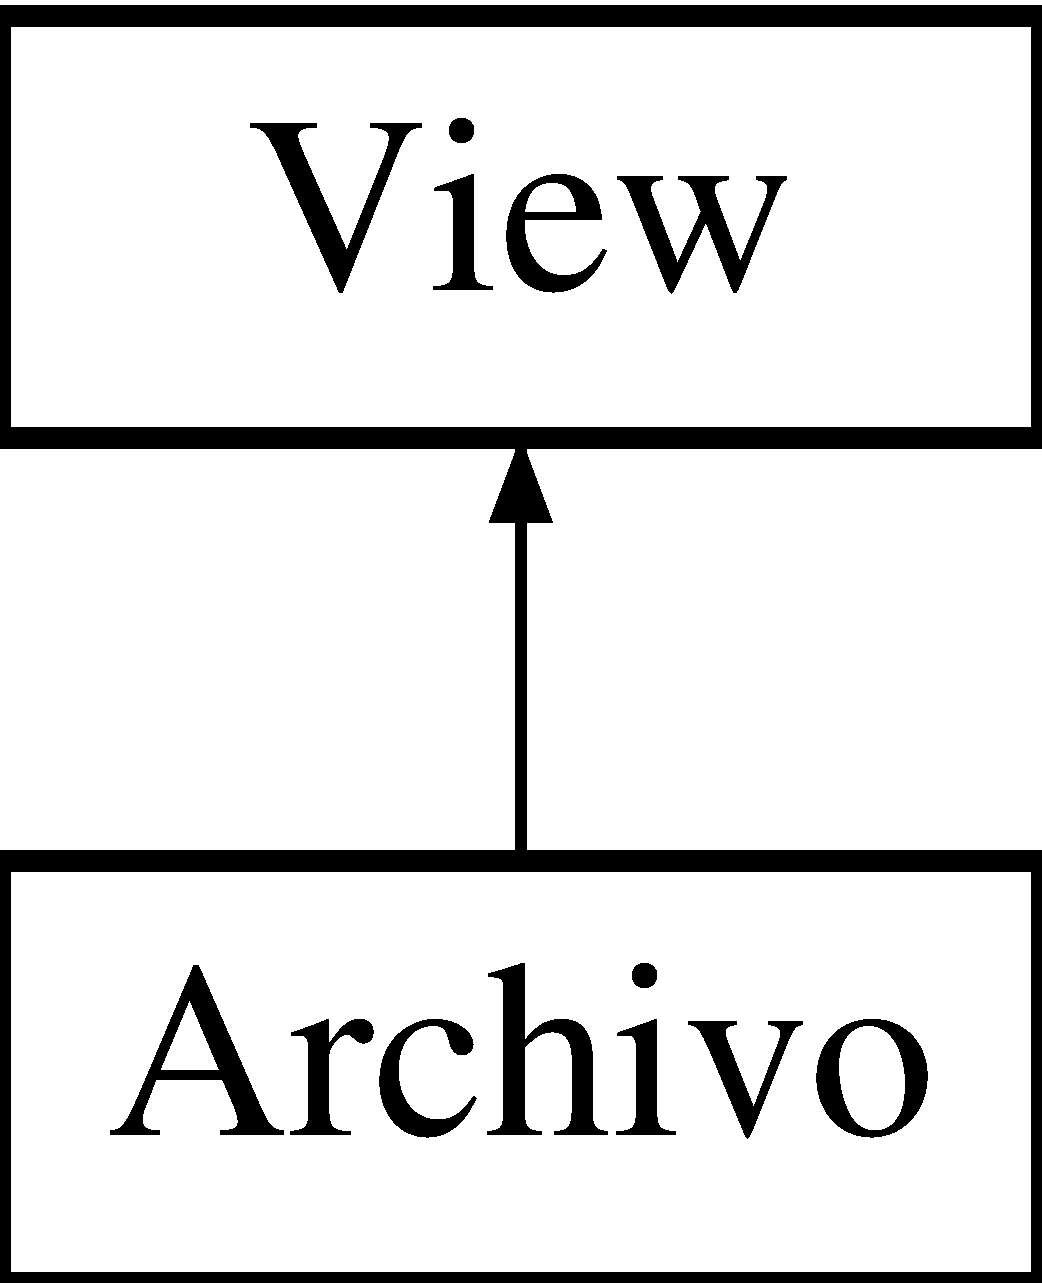
\includegraphics[height=2.000000cm]{class_archivo}
\end{center}
\end{figure}
\subsection*{Public Member Functions}
\begin{DoxyCompactItemize}
\item 
\hyperlink{class_archivo_a0adea0477e973c3e90c34b487d39b8e6}{Archivo} ()\hypertarget{class_archivo_a0adea0477e973c3e90c34b487d39b8e6}{}\label{class_archivo_a0adea0477e973c3e90c34b487d39b8e6}

\begin{DoxyCompactList}\small\item\em Constructor. \end{DoxyCompactList}\item 
\hyperlink{class_archivo_af3a49e41f903ece334f8f597dceca6f1}{$\sim$\+Archivo} ()\hypertarget{class_archivo_af3a49e41f903ece334f8f597dceca6f1}{}\label{class_archivo_af3a49e41f903ece334f8f597dceca6f1}

\begin{DoxyCompactList}\small\item\em Destructor. \end{DoxyCompactList}\item 
virtual char $\ast$ \hyperlink{class_archivo_ae92d946bce2234d8afd4cbd66f17a120}{input} (char $\ast$)
\begin{DoxyCompactList}\small\item\em Devuelve N\+U\+LL. \end{DoxyCompactList}\item 
virtual void \hyperlink{class_archivo_ad90221331fb1b3546e15158338c2b789}{output} (char $\ast$)
\begin{DoxyCompactList}\small\item\em Escribe en el archivo msj tipo char $\ast$. \end{DoxyCompactList}\item 
virtual int \hyperlink{class_archivo_a5489d20a947004f39885d42bb794b4c1}{input\+Int} (char $\ast$)
\begin{DoxyCompactList}\small\item\em Devuelve N\+U\+LL. \end{DoxyCompactList}\item 
virtual char \hyperlink{class_archivo_a5deafd974e4ed6f6416576c1076c0de8}{input\+Char} (char $\ast$)
\begin{DoxyCompactList}\small\item\em Devuelve N\+U\+LL. \end{DoxyCompactList}\item 
virtual void \hyperlink{class_archivo_acacb6d58f33e9c962b4cc8f8fb27703f}{output\+Int} (int)
\begin{DoxyCompactList}\small\item\em Escribe en el archivo msj tipo int $\ast$. \end{DoxyCompactList}\item 
virtual void \hyperlink{class_archivo_a46ab06b1dd4e3fc59b8bfc28c6ad3f3a}{output\+Char} (char)
\begin{DoxyCompactList}\small\item\em Escribe en el archivo msj tipo char. \end{DoxyCompactList}\end{DoxyCompactItemize}


\subsection{Detailed Description}
Metodos de \hyperlink{class_archivo}{Archivo}. Hija de \hyperlink{class_view}{View}. 

\subsection{Member Function Documentation}
\index{Archivo@{Archivo}!input@{input}}
\index{input@{input}!Archivo@{Archivo}}
\subsubsection[{\texorpdfstring{input(char $\ast$)}{input(char *)}}]{\setlength{\rightskip}{0pt plus 5cm}char $\ast$ Archivo\+::input (
\begin{DoxyParamCaption}
\item[{char $\ast$}]{msj}
\end{DoxyParamCaption}
)\hspace{0.3cm}{\ttfamily [virtual]}}\hypertarget{class_archivo_ae92d946bce2234d8afd4cbd66f17a120}{}\label{class_archivo_ae92d946bce2234d8afd4cbd66f17a120}


Devuelve N\+U\+LL. 


\begin{DoxyParams}{Parameters}
{\em msj} & char $\ast$ \\
\hline
\end{DoxyParams}
\begin{DoxyReturn}{Returns}
N\+U\+LL 
\end{DoxyReturn}


Implements \hyperlink{class_view}{View}.

\index{Archivo@{Archivo}!input\+Char@{input\+Char}}
\index{input\+Char@{input\+Char}!Archivo@{Archivo}}
\subsubsection[{\texorpdfstring{input\+Char(char $\ast$)}{inputChar(char *)}}]{\setlength{\rightskip}{0pt plus 5cm}char Archivo\+::input\+Char (
\begin{DoxyParamCaption}
\item[{char $\ast$}]{msj}
\end{DoxyParamCaption}
)\hspace{0.3cm}{\ttfamily [virtual]}}\hypertarget{class_archivo_a5deafd974e4ed6f6416576c1076c0de8}{}\label{class_archivo_a5deafd974e4ed6f6416576c1076c0de8}


Devuelve N\+U\+LL. 


\begin{DoxyParams}{Parameters}
{\em msj} & char $\ast$ \\
\hline
\end{DoxyParams}
\begin{DoxyReturn}{Returns}
N\+U\+LL 
\end{DoxyReturn}


Implements \hyperlink{class_view}{View}.

\index{Archivo@{Archivo}!input\+Int@{input\+Int}}
\index{input\+Int@{input\+Int}!Archivo@{Archivo}}
\subsubsection[{\texorpdfstring{input\+Int(char $\ast$)}{inputInt(char *)}}]{\setlength{\rightskip}{0pt plus 5cm}int Archivo\+::input\+Int (
\begin{DoxyParamCaption}
\item[{char $\ast$}]{msj}
\end{DoxyParamCaption}
)\hspace{0.3cm}{\ttfamily [virtual]}}\hypertarget{class_archivo_a5489d20a947004f39885d42bb794b4c1}{}\label{class_archivo_a5489d20a947004f39885d42bb794b4c1}


Devuelve N\+U\+LL. 


\begin{DoxyParams}{Parameters}
{\em msj} & char $\ast$ \\
\hline
\end{DoxyParams}
\begin{DoxyReturn}{Returns}
N\+U\+LL 
\end{DoxyReturn}


Implements \hyperlink{class_view}{View}.

\index{Archivo@{Archivo}!output@{output}}
\index{output@{output}!Archivo@{Archivo}}
\subsubsection[{\texorpdfstring{output(char $\ast$)}{output(char *)}}]{\setlength{\rightskip}{0pt plus 5cm}void Archivo\+::output (
\begin{DoxyParamCaption}
\item[{char $\ast$}]{msj}
\end{DoxyParamCaption}
)\hspace{0.3cm}{\ttfamily [virtual]}}\hypertarget{class_archivo_ad90221331fb1b3546e15158338c2b789}{}\label{class_archivo_ad90221331fb1b3546e15158338c2b789}


Escribe en el archivo msj tipo char $\ast$. 


\begin{DoxyParams}{Parameters}
{\em msj} & char $\ast$ \\
\hline
\end{DoxyParams}


Implements \hyperlink{class_view}{View}.

\index{Archivo@{Archivo}!output\+Char@{output\+Char}}
\index{output\+Char@{output\+Char}!Archivo@{Archivo}}
\subsubsection[{\texorpdfstring{output\+Char(char)}{outputChar(char)}}]{\setlength{\rightskip}{0pt plus 5cm}void Archivo\+::output\+Char (
\begin{DoxyParamCaption}
\item[{char}]{c}
\end{DoxyParamCaption}
)\hspace{0.3cm}{\ttfamily [virtual]}}\hypertarget{class_archivo_a46ab06b1dd4e3fc59b8bfc28c6ad3f3a}{}\label{class_archivo_a46ab06b1dd4e3fc59b8bfc28c6ad3f3a}


Escribe en el archivo msj tipo char. 


\begin{DoxyParams}{Parameters}
{\em c} & char \\
\hline
\end{DoxyParams}


Implements \hyperlink{class_view}{View}.

\index{Archivo@{Archivo}!output\+Int@{output\+Int}}
\index{output\+Int@{output\+Int}!Archivo@{Archivo}}
\subsubsection[{\texorpdfstring{output\+Int(int)}{outputInt(int)}}]{\setlength{\rightskip}{0pt plus 5cm}void Archivo\+::output\+Int (
\begin{DoxyParamCaption}
\item[{int}]{i}
\end{DoxyParamCaption}
)\hspace{0.3cm}{\ttfamily [virtual]}}\hypertarget{class_archivo_acacb6d58f33e9c962b4cc8f8fb27703f}{}\label{class_archivo_acacb6d58f33e9c962b4cc8f8fb27703f}


Escribe en el archivo msj tipo int $\ast$. 


\begin{DoxyParams}{Parameters}
{\em msj} & int \\
\hline
\end{DoxyParams}


Implements \hyperlink{class_view}{View}.



The documentation for this class was generated from the following files\+:\begin{DoxyCompactItemize}
\item 
C\+:/\+Users/\+Alexa Duarte/\+Desktop/\+Examen\+I-\/\+Juegos\+Y\+Jugadores\+Polimorficos/\+Examen\+I-\/\+Juegos\+Y\+Jugadores\+Polimorficos/Archivo.\+h\item 
C\+:/\+Users/\+Alexa Duarte/\+Desktop/\+Examen\+I-\/\+Juegos\+Y\+Jugadores\+Polimorficos/\+Examen\+I-\/\+Juegos\+Y\+Jugadores\+Polimorficos/Archivo.\+cpp\end{DoxyCompactItemize}

\hypertarget{class_carta}{}\section{Carta Class Reference}
\label{class_carta}\index{Carta@{Carta}}


Crea cartas.  




{\ttfamily \#include $<$Carta.\+h$>$}

\subsection*{Public Member Functions}
\begin{DoxyCompactItemize}
\item 
\hyperlink{class_carta_aa200fdc7aade3354cc2a27c1bd53a874}{Carta} (int)
\begin{DoxyCompactList}\small\item\em Constructor. \end{DoxyCompactList}\item 
\hyperlink{class_carta_ae3f30ed1ac1712b56330186f9e2139ec}{$\sim$\+Carta} ()\hypertarget{class_carta_ae3f30ed1ac1712b56330186f9e2139ec}{}\label{class_carta_ae3f30ed1ac1712b56330186f9e2139ec}

\begin{DoxyCompactList}\small\item\em Destructor. \end{DoxyCompactList}\item 
int \hyperlink{class_carta_a2455a2975994b4ff045ef254a09a1650}{get\+Numero} ()
\begin{DoxyCompactList}\small\item\em Devuelve numero de carta. \end{DoxyCompactList}\end{DoxyCompactItemize}


\subsection{Detailed Description}
Crea cartas. 

\subsection{Constructor \& Destructor Documentation}
\index{Carta@{Carta}!Carta@{Carta}}
\index{Carta@{Carta}!Carta@{Carta}}
\subsubsection[{\texorpdfstring{Carta(int)}{Carta(int)}}]{\setlength{\rightskip}{0pt plus 5cm}Carta\+::\+Carta (
\begin{DoxyParamCaption}
\item[{int}]{numero}
\end{DoxyParamCaption}
)}\hypertarget{class_carta_aa200fdc7aade3354cc2a27c1bd53a874}{}\label{class_carta_aa200fdc7aade3354cc2a27c1bd53a874}


Constructor. 


\begin{DoxyParams}{Parameters}
{\em numero} & int. Numero de carta. \\
\hline
\end{DoxyParams}


\subsection{Member Function Documentation}
\index{Carta@{Carta}!get\+Numero@{get\+Numero}}
\index{get\+Numero@{get\+Numero}!Carta@{Carta}}
\subsubsection[{\texorpdfstring{get\+Numero()}{getNumero()}}]{\setlength{\rightskip}{0pt plus 5cm}int Carta\+::get\+Numero (
\begin{DoxyParamCaption}
{}
\end{DoxyParamCaption}
)}\hypertarget{class_carta_a2455a2975994b4ff045ef254a09a1650}{}\label{class_carta_a2455a2975994b4ff045ef254a09a1650}


Devuelve numero de carta. 

\begin{DoxyReturn}{Returns}
int numero. Numero de carta. 
\end{DoxyReturn}


The documentation for this class was generated from the following files\+:\begin{DoxyCompactItemize}
\item 
C\+:/\+Users/\+Alexa Duarte/\+Desktop/\+Examen\+I-\/\+Juegos\+Y\+Jugadores\+Polimorficos/\+Examen\+I-\/\+Juegos\+Y\+Jugadores\+Polimorficos/Carta.\+h\item 
C\+:/\+Users/\+Alexa Duarte/\+Desktop/\+Examen\+I-\/\+Juegos\+Y\+Jugadores\+Polimorficos/\+Examen\+I-\/\+Juegos\+Y\+Jugadores\+Polimorficos/Carta.\+cpp\end{DoxyCompactItemize}

\hypertarget{class_consola}{}\section{Consola Class Reference}
\label{class_consola}\index{Consola@{Consola}}


Metodos de \hyperlink{class_consola}{Consola}. Hija de \hyperlink{class_view}{View}.  




{\ttfamily \#include $<$Consola.\+h$>$}

Inheritance diagram for Consola\+:\begin{figure}[H]
\begin{center}
\leavevmode
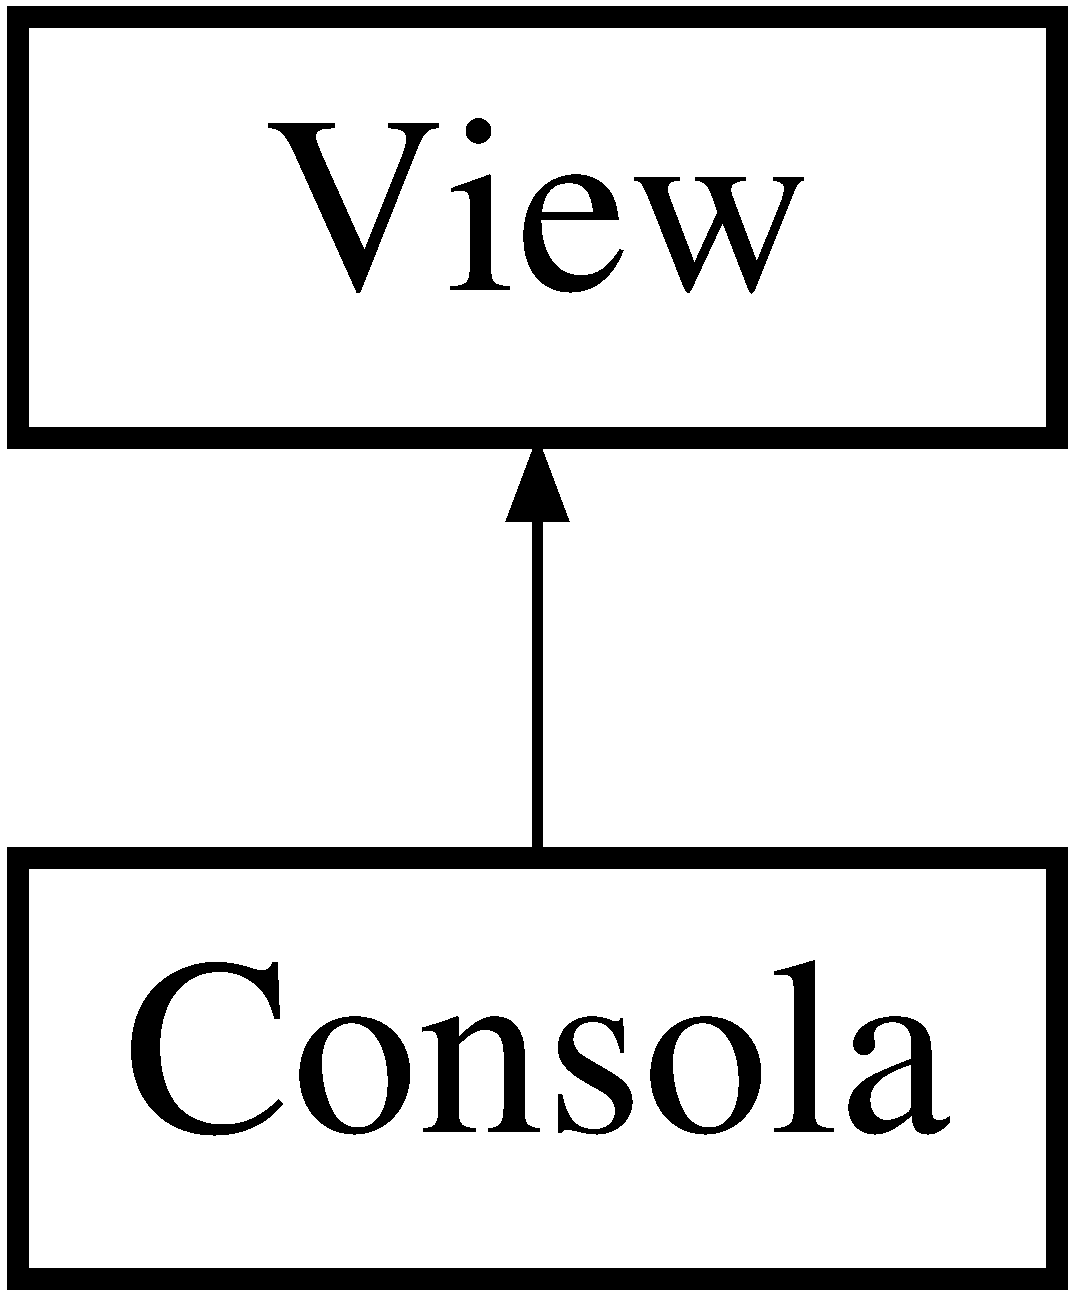
\includegraphics[height=2.000000cm]{class_consola}
\end{center}
\end{figure}
\subsection*{Public Member Functions}
\begin{DoxyCompactItemize}
\item 
\hyperlink{class_consola_a3ff916630eb67f128d522b870ae6c439}{Consola} ()\hypertarget{class_consola_a3ff916630eb67f128d522b870ae6c439}{}\label{class_consola_a3ff916630eb67f128d522b870ae6c439}

\begin{DoxyCompactList}\small\item\em Constructor. \end{DoxyCompactList}\item 
virtual \hyperlink{class_consola_a6fa096bc9af905959000b7b33a564af9}{$\sim$\+Consola} ()\hypertarget{class_consola_a6fa096bc9af905959000b7b33a564af9}{}\label{class_consola_a6fa096bc9af905959000b7b33a564af9}

\begin{DoxyCompactList}\small\item\em Destructor. \end{DoxyCompactList}\item 
virtual char $\ast$ \hyperlink{class_consola_a7841aab76efc1455db0f70150da9ac9f}{input} (char $\ast$)
\begin{DoxyCompactList}\small\item\em Devuelve imput tipo char $\ast$. \end{DoxyCompactList}\item 
virtual int \hyperlink{class_consola_a550878e0eafe9d8aa606d43b80a7c93f}{input\+Int} (char $\ast$)
\begin{DoxyCompactList}\small\item\em Devuelve imput tipo int. \end{DoxyCompactList}\item 
virtual char \hyperlink{class_consola_a1645e6ac0a93033bcd126f71c2092a94}{input\+Char} (char $\ast$)
\begin{DoxyCompactList}\small\item\em Devuelve imput tipo char. \end{DoxyCompactList}\item 
virtual void \hyperlink{class_consola_a7655c767964f53f3ff18bf2c184b1ec3}{output} (char $\ast$)
\begin{DoxyCompactList}\small\item\em Imprime mensaje. \end{DoxyCompactList}\item 
virtual void \hyperlink{class_consola_ab8cde9154436a0d47d6690fb1bc69f5c}{output\+Int} (int)
\begin{DoxyCompactList}\small\item\em Imprime mensaje. \end{DoxyCompactList}\item 
virtual void \hyperlink{class_consola_a455f9dfe7855f3107373fc03d1ee75e2}{output\+Char} (char)
\begin{DoxyCompactList}\small\item\em Imprime mensaje. \end{DoxyCompactList}\end{DoxyCompactItemize}


\subsection{Detailed Description}
Metodos de \hyperlink{class_consola}{Consola}. Hija de \hyperlink{class_view}{View}. 

\subsection{Member Function Documentation}
\index{Consola@{Consola}!input@{input}}
\index{input@{input}!Consola@{Consola}}
\subsubsection[{\texorpdfstring{input(char $\ast$)}{input(char *)}}]{\setlength{\rightskip}{0pt plus 5cm}char $\ast$ Consola\+::input (
\begin{DoxyParamCaption}
\item[{char $\ast$}]{mensaje}
\end{DoxyParamCaption}
)\hspace{0.3cm}{\ttfamily [virtual]}}\hypertarget{class_consola_a7841aab76efc1455db0f70150da9ac9f}{}\label{class_consola_a7841aab76efc1455db0f70150da9ac9f}


Devuelve imput tipo char $\ast$. 


\begin{DoxyParams}{Parameters}
{\em mensaje} & char $\ast$ \\
\hline
\end{DoxyParams}
\begin{DoxyReturn}{Returns}
in char $\ast$ 
\end{DoxyReturn}


Implements \hyperlink{class_view}{View}.

\index{Consola@{Consola}!input\+Char@{input\+Char}}
\index{input\+Char@{input\+Char}!Consola@{Consola}}
\subsubsection[{\texorpdfstring{input\+Char(char $\ast$)}{inputChar(char *)}}]{\setlength{\rightskip}{0pt plus 5cm}char Consola\+::input\+Char (
\begin{DoxyParamCaption}
\item[{char $\ast$}]{mensaje}
\end{DoxyParamCaption}
)\hspace{0.3cm}{\ttfamily [virtual]}}\hypertarget{class_consola_a1645e6ac0a93033bcd126f71c2092a94}{}\label{class_consola_a1645e6ac0a93033bcd126f71c2092a94}


Devuelve imput tipo char. 


\begin{DoxyParams}{Parameters}
{\em mensaje} & char $\ast$ \\
\hline
\end{DoxyParams}
\begin{DoxyReturn}{Returns}
in char 
\end{DoxyReturn}


Implements \hyperlink{class_view}{View}.

\index{Consola@{Consola}!input\+Int@{input\+Int}}
\index{input\+Int@{input\+Int}!Consola@{Consola}}
\subsubsection[{\texorpdfstring{input\+Int(char $\ast$)}{inputInt(char *)}}]{\setlength{\rightskip}{0pt plus 5cm}int Consola\+::input\+Int (
\begin{DoxyParamCaption}
\item[{char $\ast$}]{mensaje}
\end{DoxyParamCaption}
)\hspace{0.3cm}{\ttfamily [virtual]}}\hypertarget{class_consola_a550878e0eafe9d8aa606d43b80a7c93f}{}\label{class_consola_a550878e0eafe9d8aa606d43b80a7c93f}


Devuelve imput tipo int. 


\begin{DoxyParams}{Parameters}
{\em mensaje} & char $\ast$ \\
\hline
\end{DoxyParams}
\begin{DoxyReturn}{Returns}
in int 
\end{DoxyReturn}


Implements \hyperlink{class_view}{View}.

\index{Consola@{Consola}!output@{output}}
\index{output@{output}!Consola@{Consola}}
\subsubsection[{\texorpdfstring{output(char $\ast$)}{output(char *)}}]{\setlength{\rightskip}{0pt plus 5cm}void Consola\+::output (
\begin{DoxyParamCaption}
\item[{char $\ast$}]{mensaje}
\end{DoxyParamCaption}
)\hspace{0.3cm}{\ttfamily [virtual]}}\hypertarget{class_consola_a7655c767964f53f3ff18bf2c184b1ec3}{}\label{class_consola_a7655c767964f53f3ff18bf2c184b1ec3}


Imprime mensaje. 


\begin{DoxyParams}{Parameters}
{\em mensaje} & char $\ast$ \\
\hline
\end{DoxyParams}


Implements \hyperlink{class_view}{View}.

\index{Consola@{Consola}!output\+Char@{output\+Char}}
\index{output\+Char@{output\+Char}!Consola@{Consola}}
\subsubsection[{\texorpdfstring{output\+Char(char)}{outputChar(char)}}]{\setlength{\rightskip}{0pt plus 5cm}void Consola\+::output\+Char (
\begin{DoxyParamCaption}
\item[{char}]{c}
\end{DoxyParamCaption}
)\hspace{0.3cm}{\ttfamily [virtual]}}\hypertarget{class_consola_a455f9dfe7855f3107373fc03d1ee75e2}{}\label{class_consola_a455f9dfe7855f3107373fc03d1ee75e2}


Imprime mensaje. 


\begin{DoxyParams}{Parameters}
{\em mensaje} & char \\
\hline
\end{DoxyParams}


Implements \hyperlink{class_view}{View}.

\index{Consola@{Consola}!output\+Int@{output\+Int}}
\index{output\+Int@{output\+Int}!Consola@{Consola}}
\subsubsection[{\texorpdfstring{output\+Int(int)}{outputInt(int)}}]{\setlength{\rightskip}{0pt plus 5cm}void Consola\+::output\+Int (
\begin{DoxyParamCaption}
\item[{int}]{i}
\end{DoxyParamCaption}
)\hspace{0.3cm}{\ttfamily [virtual]}}\hypertarget{class_consola_ab8cde9154436a0d47d6690fb1bc69f5c}{}\label{class_consola_ab8cde9154436a0d47d6690fb1bc69f5c}


Imprime mensaje. 


\begin{DoxyParams}{Parameters}
{\em mensaje} & int \\
\hline
\end{DoxyParams}


Implements \hyperlink{class_view}{View}.



The documentation for this class was generated from the following files\+:\begin{DoxyCompactItemize}
\item 
C\+:/\+Users/\+Alexa Duarte/\+Desktop/\+Examen\+I-\/\+Juegos\+Y\+Jugadores\+Polimorficos/\+Examen\+I-\/\+Juegos\+Y\+Jugadores\+Polimorficos/Consola.\+h\item 
C\+:/\+Users/\+Alexa Duarte/\+Desktop/\+Examen\+I-\/\+Juegos\+Y\+Jugadores\+Polimorficos/\+Examen\+I-\/\+Juegos\+Y\+Jugadores\+Polimorficos/Consola.\+cpp\end{DoxyCompactItemize}

\hypertarget{class_controller}{}\section{Controller Class Reference}
\label{class_controller}\index{Controller@{Controller}}


Controlador de las clases.  




{\ttfamily \#include $<$Controller.\+h$>$}

\subsection*{Public Member Functions}
\begin{DoxyCompactItemize}
\item 
\hyperlink{class_controller_a95c56822d667e94b031451729ce069a9}{Controller} ()\hypertarget{class_controller_a95c56822d667e94b031451729ce069a9}{}\label{class_controller_a95c56822d667e94b031451729ce069a9}

\begin{DoxyCompactList}\small\item\em Constructor. Crea objeto \hyperlink{class_model}{Model} y objetos de \hyperlink{class_view}{View}. \end{DoxyCompactList}\item 
\hyperlink{class_controller_a0ab87934c4f7a266cfdb86e0f36bc1b5}{$\sim$\+Controller} ()\hypertarget{class_controller_a0ab87934c4f7a266cfdb86e0f36bc1b5}{}\label{class_controller_a0ab87934c4f7a266cfdb86e0f36bc1b5}

\begin{DoxyCompactList}\small\item\em Desctructor. \end{DoxyCompactList}\item 
void \hyperlink{class_controller_ab8808d4fd327fb37d6bcf8eba1f2da6c}{iniciar} ()\hypertarget{class_controller_ab8808d4fd327fb37d6bcf8eba1f2da6c}{}\label{class_controller_ab8808d4fd327fb37d6bcf8eba1f2da6c}

\begin{DoxyCompactList}\small\item\em Inicia el programa. \end{DoxyCompactList}\end{DoxyCompactItemize}


\subsection{Detailed Description}
Controlador de las clases. 

The documentation for this class was generated from the following files\+:\begin{DoxyCompactItemize}
\item 
C\+:/\+Users/\+Alexa Duarte/\+Desktop/\+Examen\+I-\/\+Juegos\+Y\+Jugadores\+Polimorficos/\+Examen\+I-\/\+Juegos\+Y\+Jugadores\+Polimorficos/Controller.\+h\item 
C\+:/\+Users/\+Alexa Duarte/\+Desktop/\+Examen\+I-\/\+Juegos\+Y\+Jugadores\+Polimorficos/\+Examen\+I-\/\+Juegos\+Y\+Jugadores\+Polimorficos/Controller.\+cpp\end{DoxyCompactItemize}

\hypertarget{class_deck}{}\section{Deck Class Reference}
\label{class_deck}\index{Deck@{Deck}}


Crea deck de cartas.  




{\ttfamily \#include $<$Deck.\+h$>$}

\subsection*{Public Member Functions}
\begin{DoxyCompactItemize}
\item 
\hyperlink{class_deck_a57ae1cb4ac6fd61c249cefb2db85eb99}{Deck} ()\hypertarget{class_deck_a57ae1cb4ac6fd61c249cefb2db85eb99}{}\label{class_deck_a57ae1cb4ac6fd61c249cefb2db85eb99}

\begin{DoxyCompactList}\small\item\em Constructor. \end{DoxyCompactList}\item 
virtual \hyperlink{class_deck_a7d1331cc558c302fdf44e5ae8aae1a95}{$\sim$\+Deck} ()\hypertarget{class_deck_a7d1331cc558c302fdf44e5ae8aae1a95}{}\label{class_deck_a7d1331cc558c302fdf44e5ae8aae1a95}

\begin{DoxyCompactList}\small\item\em Destructor. Borra cartas de la lista. \end{DoxyCompactList}\item 
\hyperlink{class_carta}{Carta} $\ast$ \hyperlink{class_deck_a1f65a1dde03b592f8e74700635f31af7}{obtener\+Carta} ()
\begin{DoxyCompactList}\small\item\em Devuelve una carta de la baraja para ser repartida y la elimina del deck. \end{DoxyCompactList}\end{DoxyCompactItemize}


\subsection{Detailed Description}
Crea deck de cartas. 

\subsection{Member Function Documentation}
\index{Deck@{Deck}!obtener\+Carta@{obtener\+Carta}}
\index{obtener\+Carta@{obtener\+Carta}!Deck@{Deck}}
\subsubsection[{\texorpdfstring{obtener\+Carta()}{obtenerCarta()}}]{\setlength{\rightskip}{0pt plus 5cm}{\bf Carta} $\ast$ Deck\+::obtener\+Carta (
\begin{DoxyParamCaption}
{}
\end{DoxyParamCaption}
)}\hypertarget{class_deck_a1f65a1dde03b592f8e74700635f31af7}{}\label{class_deck_a1f65a1dde03b592f8e74700635f31af7}


Devuelve una carta de la baraja para ser repartida y la elimina del deck. 

\begin{DoxyReturn}{Returns}
\hyperlink{class_carta}{Carta} $\ast$. \hyperlink{class_carta}{Carta} de la baraja. 
\end{DoxyReturn}


The documentation for this class was generated from the following files\+:\begin{DoxyCompactItemize}
\item 
C\+:/\+Users/\+Alexa Duarte/\+Desktop/\+Examen\+I-\/\+Juegos\+Y\+Jugadores\+Polimorficos/\+Examen\+I-\/\+Juegos\+Y\+Jugadores\+Polimorficos/Deck.\+h\item 
C\+:/\+Users/\+Alexa Duarte/\+Desktop/\+Examen\+I-\/\+Juegos\+Y\+Jugadores\+Polimorficos/\+Examen\+I-\/\+Juegos\+Y\+Jugadores\+Polimorficos/Deck.\+cpp\end{DoxyCompactItemize}

\hypertarget{class_juego}{}\section{Juego Class Reference}
\label{class_juego}\index{Juego@{Juego}}


Clase puramente virtual. Hija de modelo.  




{\ttfamily \#include $<$Juego.\+h$>$}

Inheritance diagram for Juego\+:\begin{figure}[H]
\begin{center}
\leavevmode
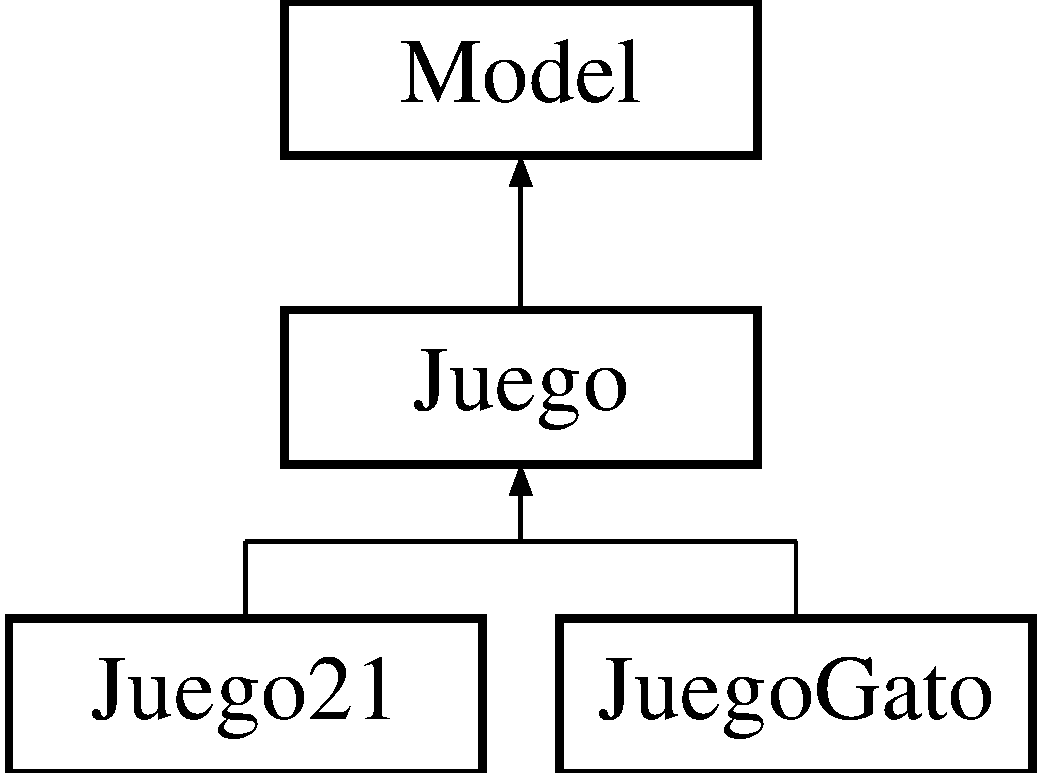
\includegraphics[height=3.000000cm]{class_juego}
\end{center}
\end{figure}
\subsection*{Public Member Functions}
\begin{DoxyCompactItemize}
\item 
virtual void \hyperlink{class_juego_a92053738ca2f7375ef42211a72e59f5c}{terminar\+Juego} ()=0
\item 
virtual void \hyperlink{class_juego_aa2906c1f0ae10f2f34cd49f52bdd14ed}{jugar} ()=0
\end{DoxyCompactItemize}
\subsection*{Protected Member Functions}
\begin{DoxyCompactItemize}
\item 
virtual void {\bfseries crear\+Jugadores\+Humanos} ()=0\hypertarget{class_juego_a3edaee94e248a4f107c825965e816627}{}\label{class_juego_a3edaee94e248a4f107c825965e816627}

\item 
virtual void {\bfseries crear\+Jugadores\+Maquinas} ()=0\hypertarget{class_juego_ad0ae19cdb246e387739ccc1fe16f7c62}{}\label{class_juego_ad0ae19cdb246e387739ccc1fe16f7c62}

\item 
virtual void {\bfseries add\+Vistas} ()=0\hypertarget{class_juego_aad6ae20d1dc71102101e16e774f4e78b}{}\label{class_juego_aad6ae20d1dc71102101e16e774f4e78b}

\item 
virtual void {\bfseries mostrar} ()=0\hypertarget{class_juego_acb3cc272016f24b02813485fd4d6680e}{}\label{class_juego_acb3cc272016f24b02813485fd4d6680e}

\end{DoxyCompactItemize}
\subsection*{Additional Inherited Members}


\subsection{Detailed Description}
Clase puramente virtual. Hija de modelo. 

\subsection{Member Function Documentation}
\index{Juego@{Juego}!jugar@{jugar}}
\index{jugar@{jugar}!Juego@{Juego}}
\subsubsection[{\texorpdfstring{jugar()=0}{jugar()=0}}]{\setlength{\rightskip}{0pt plus 5cm}virtual void Juego\+::jugar (
\begin{DoxyParamCaption}
{}
\end{DoxyParamCaption}
)\hspace{0.3cm}{\ttfamily [pure virtual]}}\hypertarget{class_juego_aa2906c1f0ae10f2f34cd49f52bdd14ed}{}\label{class_juego_aa2906c1f0ae10f2f34cd49f52bdd14ed}
Inicia el juego 

Implemented in \hyperlink{class_juego_gato_a59466c4b571c4f8d571f8594565f164d}{Juego\+Gato}, and \hyperlink{class_juego21_a5b450c7b4e68d1741e3e7ed9808d4667}{Juego21}.

\index{Juego@{Juego}!terminar\+Juego@{terminar\+Juego}}
\index{terminar\+Juego@{terminar\+Juego}!Juego@{Juego}}
\subsubsection[{\texorpdfstring{terminar\+Juego()=0}{terminarJuego()=0}}]{\setlength{\rightskip}{0pt plus 5cm}virtual void Juego\+::terminar\+Juego (
\begin{DoxyParamCaption}
{}
\end{DoxyParamCaption}
)\hspace{0.3cm}{\ttfamily [pure virtual]}}\hypertarget{class_juego_a92053738ca2f7375ef42211a72e59f5c}{}\label{class_juego_a92053738ca2f7375ef42211a72e59f5c}
Destructor Finaliza el juego 

Implemented in \hyperlink{class_juego_gato_a73773d53339b0e50afc76c7806c9f142}{Juego\+Gato}, and \hyperlink{class_juego21_a5bf192fbb3bbd76717600d307065cbea}{Juego21}.



The documentation for this class was generated from the following files\+:\begin{DoxyCompactItemize}
\item 
C\+:/\+Users/\+Alexa Duarte/\+Desktop/\+Examen\+I-\/\+Juegos\+Y\+Jugadores\+Polimorficos/\+Examen\+I-\/\+Juegos\+Y\+Jugadores\+Polimorficos/Juego.\+h\item 
C\+:/\+Users/\+Alexa Duarte/\+Desktop/\+Examen\+I-\/\+Juegos\+Y\+Jugadores\+Polimorficos/\+Examen\+I-\/\+Juegos\+Y\+Jugadores\+Polimorficos/Juego.\+cpp\end{DoxyCompactItemize}

\hypertarget{class_juego21}{}\section{Juego21 Class Reference}
\label{class_juego21}\index{Juego21@{Juego21}}


Implementacion del juego 21. Hija de \hyperlink{class_juego}{Juego}.  




{\ttfamily \#include $<$Juego21.\+h$>$}

Inheritance diagram for Juego21\+:\begin{figure}[H]
\begin{center}
\leavevmode
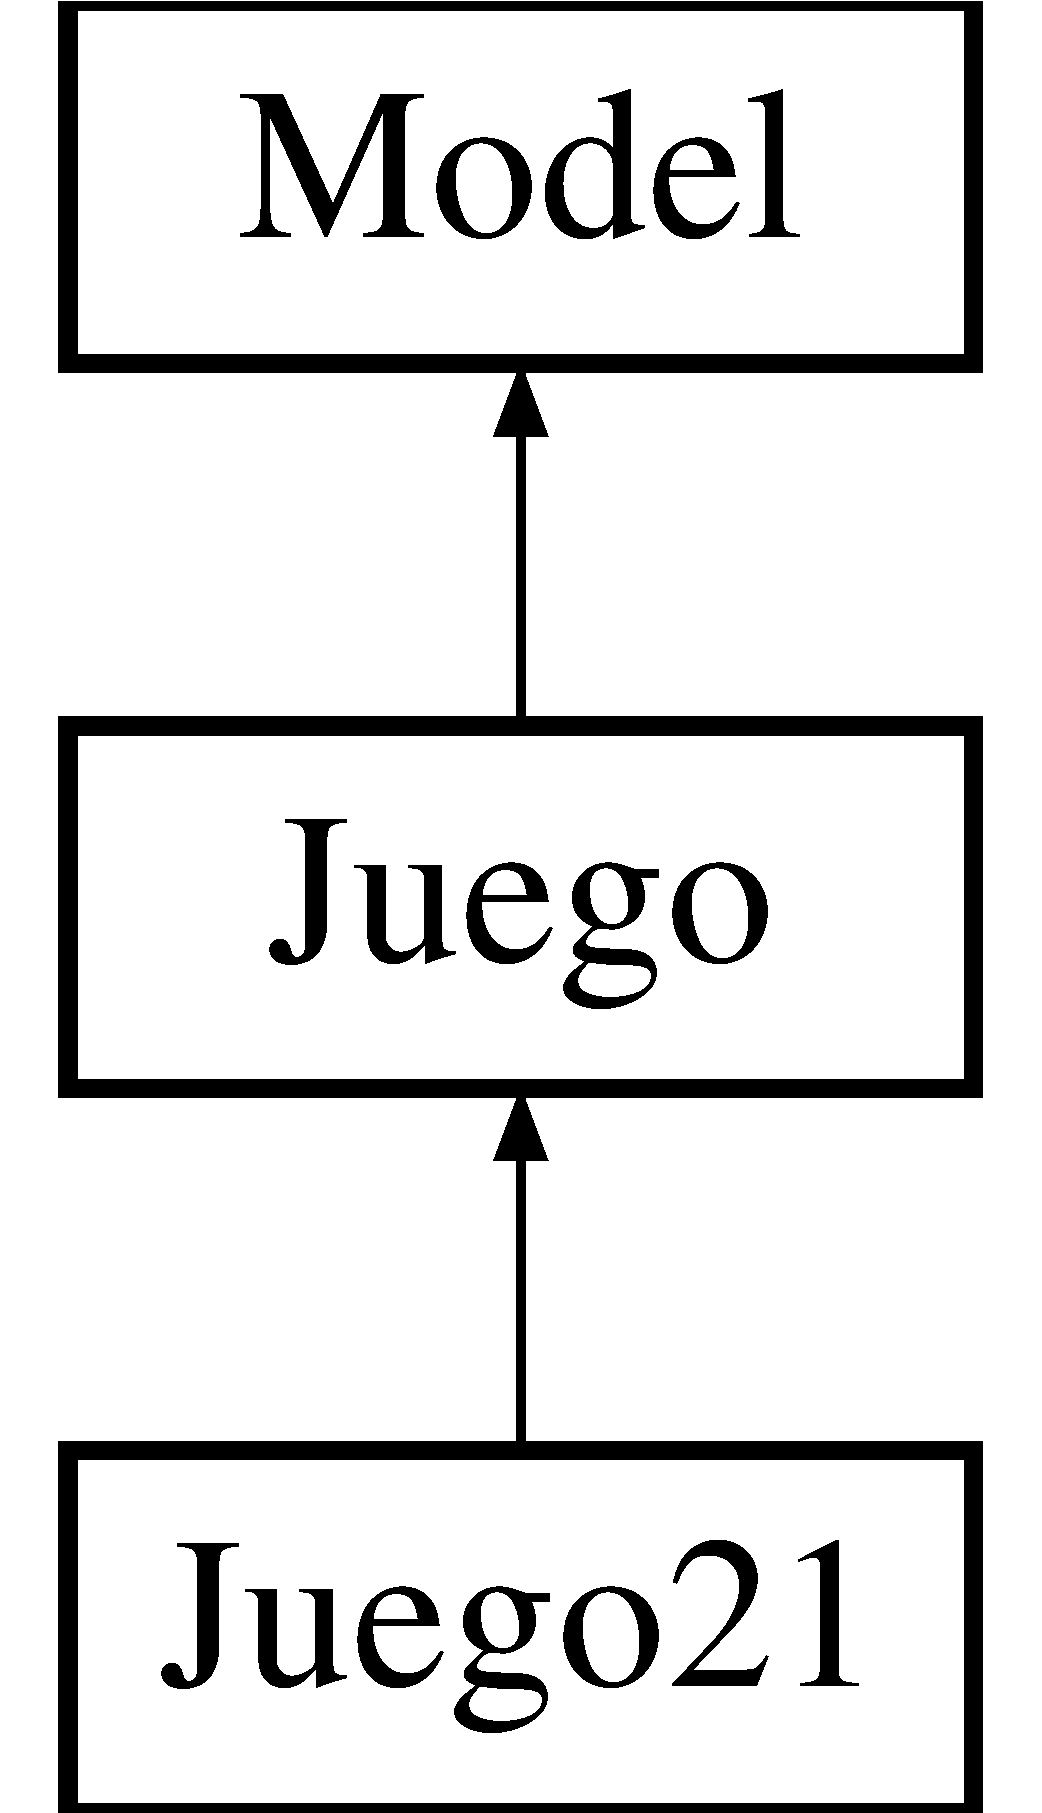
\includegraphics[height=3.000000cm]{class_juego21}
\end{center}
\end{figure}
\subsection*{Public Member Functions}
\begin{DoxyCompactItemize}
\item 
\hyperlink{class_juego21_af427a46cb9e06d7e8e3ca07281e899ef}{Juego21} ()\hypertarget{class_juego21_af427a46cb9e06d7e8e3ca07281e899ef}{}\label{class_juego21_af427a46cb9e06d7e8e3ca07281e899ef}

\begin{DoxyCompactList}\small\item\em Constructor. Crea deck de cartas. \end{DoxyCompactList}\item 
virtual \hyperlink{class_juego21_af427a347e1b7c3c12fdd4c476c61656a}{$\sim$\+Juego21} ()\hypertarget{class_juego21_af427a347e1b7c3c12fdd4c476c61656a}{}\label{class_juego21_af427a347e1b7c3c12fdd4c476c61656a}

\begin{DoxyCompactList}\small\item\em Destructor. elimina jugadores de lista y deck. \end{DoxyCompactList}\item 
virtual void \hyperlink{class_juego21_a5b450c7b4e68d1741e3e7ed9808d4667}{jugar} ()\hypertarget{class_juego21_a5b450c7b4e68d1741e3e7ed9808d4667}{}\label{class_juego21_a5b450c7b4e68d1741e3e7ed9808d4667}

\begin{DoxyCompactList}\small\item\em Inicia el juego. \end{DoxyCompactList}\item 
virtual void \hyperlink{class_juego21_a5bf192fbb3bbd76717600d307065cbea}{terminar\+Juego} ()\hypertarget{class_juego21_a5bf192fbb3bbd76717600d307065cbea}{}\label{class_juego21_a5bf192fbb3bbd76717600d307065cbea}

\begin{DoxyCompactList}\small\item\em Termina el juego y revela al ganador. \end{DoxyCompactList}\end{DoxyCompactItemize}
\subsection*{Additional Inherited Members}


\subsection{Detailed Description}
Implementacion del juego 21. Hija de \hyperlink{class_juego}{Juego}. 

The documentation for this class was generated from the following files\+:\begin{DoxyCompactItemize}
\item 
C\+:/\+Users/\+Alexa Duarte/\+Desktop/\+Examen\+I-\/\+Juegos\+Y\+Jugadores\+Polimorficos/\+Examen\+I-\/\+Juegos\+Y\+Jugadores\+Polimorficos/Juego21.\+h\item 
C\+:/\+Users/\+Alexa Duarte/\+Desktop/\+Examen\+I-\/\+Juegos\+Y\+Jugadores\+Polimorficos/\+Examen\+I-\/\+Juegos\+Y\+Jugadores\+Polimorficos/Juego21.\+cpp\end{DoxyCompactItemize}

\hypertarget{class_juego_gato}{}\section{Juego\+Gato Class Reference}
\label{class_juego_gato}\index{Juego\+Gato@{Juego\+Gato}}


Atributos y metodos del juego gato. Hija de juego.  




{\ttfamily \#include $<$Juego\+Gato.\+h$>$}

Inheritance diagram for Juego\+Gato\+:\begin{figure}[H]
\begin{center}
\leavevmode
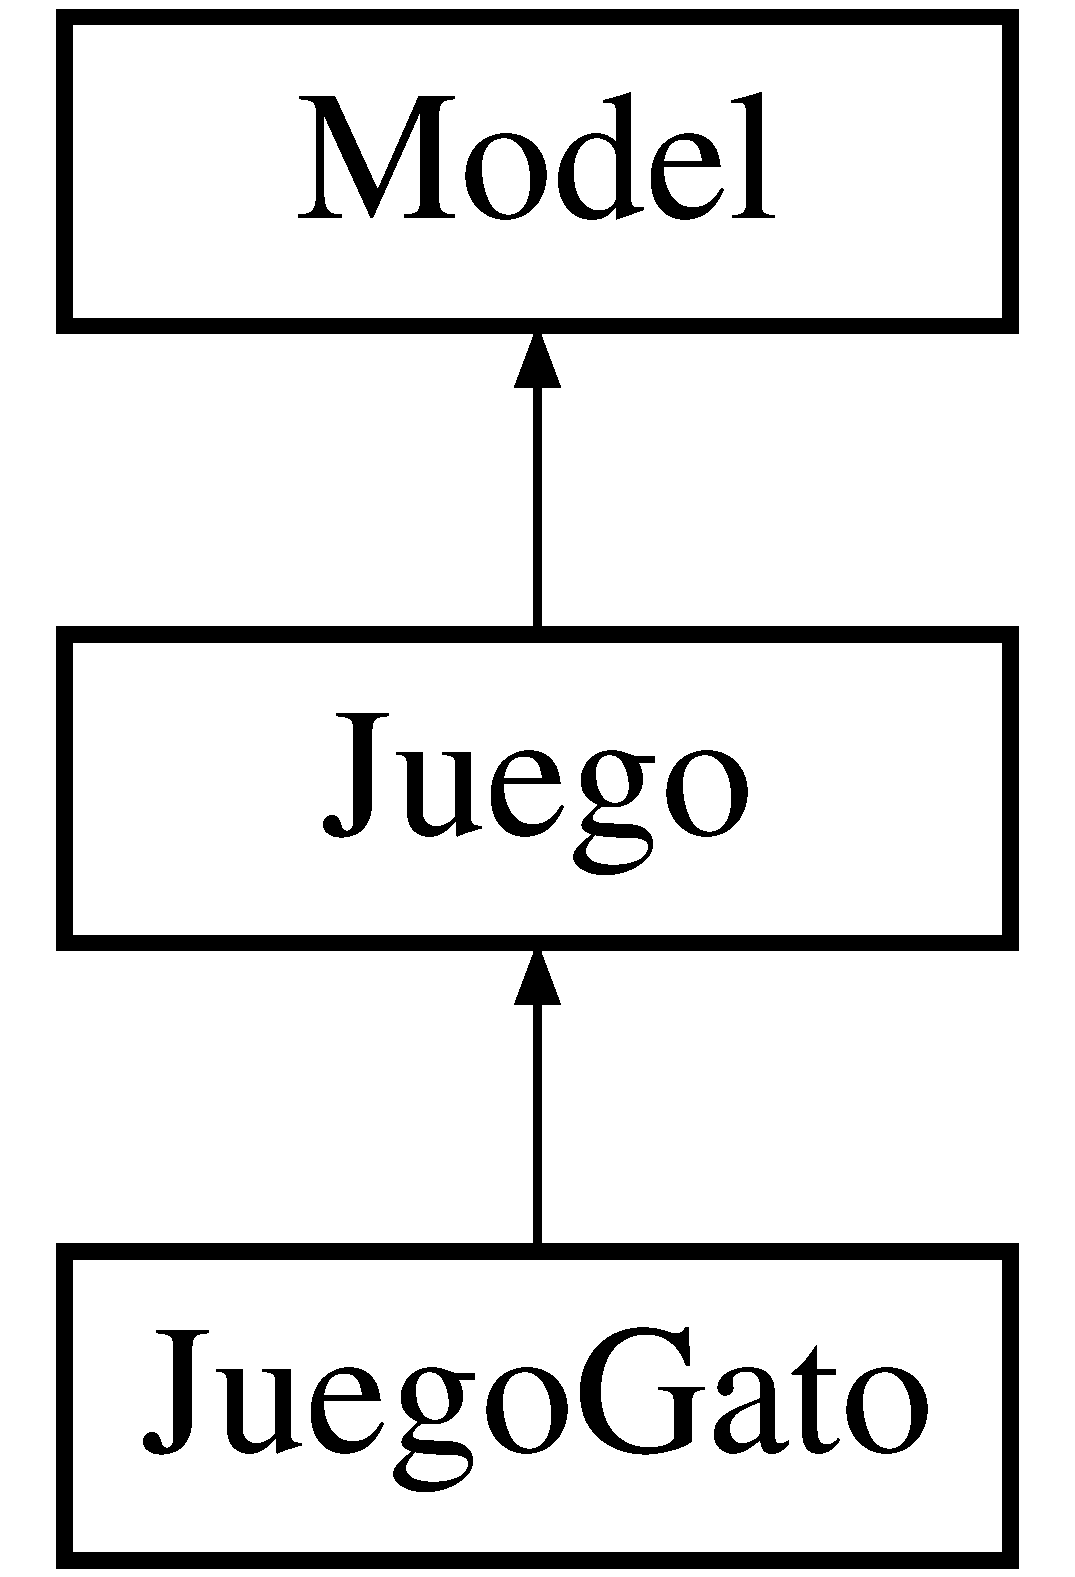
\includegraphics[height=3.000000cm]{class_juego_gato}
\end{center}
\end{figure}
\subsection*{Public Member Functions}
\begin{DoxyCompactItemize}
\item 
\hyperlink{class_juego_gato_a6b948d319360d774592c8ac0cf0071a2}{Juego\+Gato} ()\hypertarget{class_juego_gato_a6b948d319360d774592c8ac0cf0071a2}{}\label{class_juego_gato_a6b948d319360d774592c8ac0cf0071a2}

\begin{DoxyCompactList}\small\item\em Constructor. Inciliza tablero y ganador. \end{DoxyCompactList}\item 
virtual \hyperlink{class_juego_gato_a437f6521c043c739580cda9292926d5b}{$\sim$\+Juego\+Gato} ()\hypertarget{class_juego_gato_a437f6521c043c739580cda9292926d5b}{}\label{class_juego_gato_a437f6521c043c739580cda9292926d5b}

\begin{DoxyCompactList}\small\item\em Destructor. \end{DoxyCompactList}\item 
virtual void \hyperlink{class_juego_gato_a59466c4b571c4f8d571f8594565f164d}{jugar} ()\hypertarget{class_juego_gato_a59466c4b571c4f8d571f8594565f164d}{}\label{class_juego_gato_a59466c4b571c4f8d571f8594565f164d}

\begin{DoxyCompactList}\small\item\em Comienza el juego. \end{DoxyCompactList}\item 
virtual void \hyperlink{class_juego_gato_a73773d53339b0e50afc76c7806c9f142}{terminar\+Juego} ()\hypertarget{class_juego_gato_a73773d53339b0e50afc76c7806c9f142}{}\label{class_juego_gato_a73773d53339b0e50afc76c7806c9f142}

\begin{DoxyCompactList}\small\item\em Termina el juego si ya hay un ganador o el tablero esta lleno. \end{DoxyCompactList}\end{DoxyCompactItemize}
\subsection*{Additional Inherited Members}


\subsection{Detailed Description}
Atributos y metodos del juego gato. Hija de juego. 

The documentation for this class was generated from the following files\+:\begin{DoxyCompactItemize}
\item 
C\+:/\+Users/\+Alexa Duarte/\+Desktop/\+Examen\+I-\/\+Juegos\+Y\+Jugadores\+Polimorficos/\+Examen\+I-\/\+Juegos\+Y\+Jugadores\+Polimorficos/Juego\+Gato.\+h\item 
C\+:/\+Users/\+Alexa Duarte/\+Desktop/\+Examen\+I-\/\+Juegos\+Y\+Jugadores\+Polimorficos/\+Examen\+I-\/\+Juegos\+Y\+Jugadores\+Polimorficos/Juego\+Gato.\+cpp\end{DoxyCompactItemize}

\hypertarget{class_jugadas21}{}\section{Jugadas21 Class Reference}
\label{class_jugadas21}\index{Jugadas21@{Jugadas21}}


Da calificaciones segun las cartas en mano.  




{\ttfamily \#include $<$Jugadas21.\+h$>$}

\subsection*{Public Member Functions}
\begin{DoxyCompactItemize}
\item 
\hyperlink{class_jugadas21_a6b8beb81593cd510ddd0213a7d67bee5}{Jugadas21} ()\hypertarget{class_jugadas21_a6b8beb81593cd510ddd0213a7d67bee5}{}\label{class_jugadas21_a6b8beb81593cd510ddd0213a7d67bee5}

\begin{DoxyCompactList}\small\item\em Constructor. \end{DoxyCompactList}\item 
\hyperlink{class_jugadas21_a979c05f8a3ea4fb7a53443d64ea951d7}{$\sim$\+Jugadas21} ()\hypertarget{class_jugadas21_a979c05f8a3ea4fb7a53443d64ea951d7}{}\label{class_jugadas21_a979c05f8a3ea4fb7a53443d64ea951d7}

\begin{DoxyCompactList}\small\item\em Destructor. \end{DoxyCompactList}\item 
int \hyperlink{class_jugadas21_a40752229af4e2c9e5a6a50d234226abd}{obtener\+Calificacion} (list$<$ \hyperlink{class_carta}{Carta} $\ast$ $>$ mano)
\begin{DoxyCompactList}\small\item\em Devuelve la calificacion segun mano. \end{DoxyCompactList}\end{DoxyCompactItemize}


\subsection{Detailed Description}
Da calificaciones segun las cartas en mano. 

\subsection{Member Function Documentation}
\index{Jugadas21@{Jugadas21}!obtener\+Calificacion@{obtener\+Calificacion}}
\index{obtener\+Calificacion@{obtener\+Calificacion}!Jugadas21@{Jugadas21}}
\subsubsection[{\texorpdfstring{obtener\+Calificacion(list$<$ Carta $\ast$ $>$ mano)}{obtenerCalificacion(list< Carta * > mano)}}]{\setlength{\rightskip}{0pt plus 5cm}int Jugadas21\+::obtener\+Calificacion (
\begin{DoxyParamCaption}
\item[{list$<$ {\bf Carta} $\ast$ $>$}]{mano}
\end{DoxyParamCaption}
)}\hypertarget{class_jugadas21_a40752229af4e2c9e5a6a50d234226abd}{}\label{class_jugadas21_a40752229af4e2c9e5a6a50d234226abd}


Devuelve la calificacion segun mano. 


\begin{DoxyParams}{Parameters}
{\em mano} & list$<$\+Carta$\ast$$>$. Mano de cartas del jugador. \\
\hline
\end{DoxyParams}
\begin{DoxyReturn}{Returns}
calificacion int. 
\end{DoxyReturn}


The documentation for this class was generated from the following files\+:\begin{DoxyCompactItemize}
\item 
C\+:/\+Users/\+Alexa Duarte/\+Desktop/\+Examen\+I-\/\+Juegos\+Y\+Jugadores\+Polimorficos/\+Examen\+I-\/\+Juegos\+Y\+Jugadores\+Polimorficos/Jugadas21.\+h\item 
C\+:/\+Users/\+Alexa Duarte/\+Desktop/\+Examen\+I-\/\+Juegos\+Y\+Jugadores\+Polimorficos/\+Examen\+I-\/\+Juegos\+Y\+Jugadores\+Polimorficos/Jugadas21.\+cpp\end{DoxyCompactItemize}

\hypertarget{class_jugador21}{}\section{Jugador21 Class Reference}
\label{class_jugador21}\index{Jugador21@{Jugador21}}


Metodos y atributos de los jugadores en 21.  




{\ttfamily \#include $<$Jugador21.\+h$>$}

Inheritance diagram for Jugador21\+:\begin{figure}[H]
\begin{center}
\leavevmode
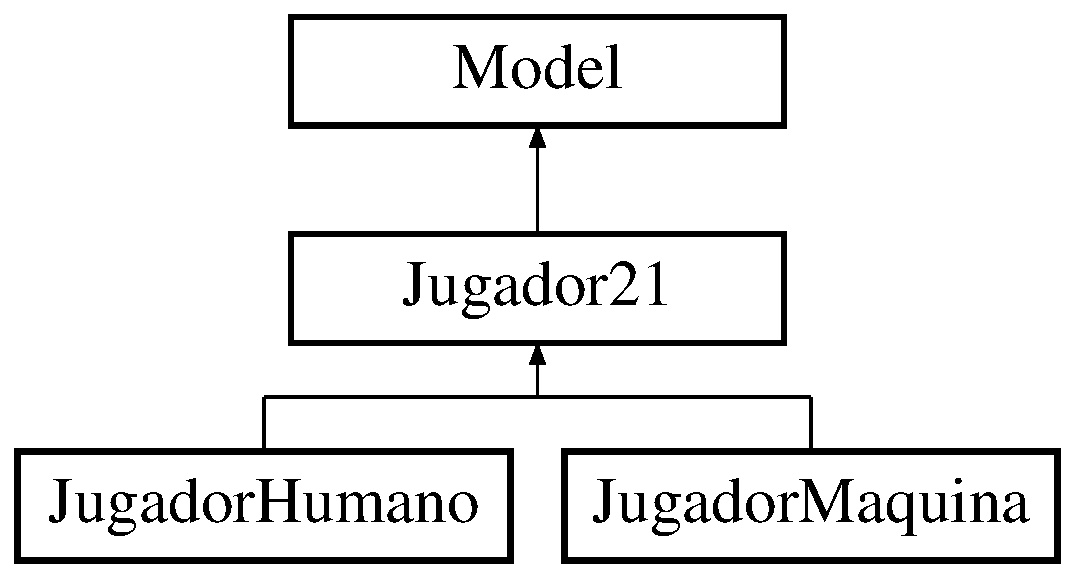
\includegraphics[height=3.000000cm]{class_jugador21}
\end{center}
\end{figure}
\subsection*{Public Member Functions}
\begin{DoxyCompactItemize}
\item 
\hyperlink{class_jugador21_a424d1aad6052177ade0cbd64daa2b4fc}{Jugador21} (char $\ast$, int)
\begin{DoxyCompactList}\small\item\em Constructor. \end{DoxyCompactList}\item 
virtual \hyperlink{class_jugador21_a59b58bf9bb8b0d25ac4b8fe1c1dd1d80}{$\sim$\+Jugador21} ()\hypertarget{class_jugador21_a59b58bf9bb8b0d25ac4b8fe1c1dd1d80}{}\label{class_jugador21_a59b58bf9bb8b0d25ac4b8fe1c1dd1d80}

\begin{DoxyCompactList}\small\item\em Destructor. \end{DoxyCompactList}\item 
list$<$ \hyperlink{class_carta}{Carta} $\ast$ $>$ \hyperlink{class_jugador21_aade6e9a04032d3a2ff4c29880f6f8739}{get\+Mano} ()
\begin{DoxyCompactList}\small\item\em Devuelve mano del jugador. \end{DoxyCompactList}\item 
void \hyperlink{class_jugador21_aa15cf22af6c5c8b11ed16944b58f878b}{anadir\+A\+Mano} (\hyperlink{class_carta}{Carta} $\ast$)
\begin{DoxyCompactList}\small\item\em Agrega carta a mano del jugador. \end{DoxyCompactList}\item 
void \hyperlink{class_jugador21_a4169f9fb97f0deb6745c23513f002ede}{set\+Puntaje} ()\hypertarget{class_jugador21_a4169f9fb97f0deb6745c23513f002ede}{}\label{class_jugador21_a4169f9fb97f0deb6745c23513f002ede}

\begin{DoxyCompactList}\small\item\em Establece el puntaje total de todas las cartas. \end{DoxyCompactList}\item 
virtual bool {\bfseries tomar\+Decision} ()=0\hypertarget{class_jugador21_aae50435712a479e360234bd932e53a72}{}\label{class_jugador21_aae50435712a479e360234bd932e53a72}

\item 
int \hyperlink{class_jugador21_a061cafa05bbbe86c083f5cb9e46064a4}{get\+Numero\+Jugador} ()
\begin{DoxyCompactList}\small\item\em Devuelve el id de jugador. \end{DoxyCompactList}\item 
char $\ast$ \hyperlink{class_jugador21_ac517b3e12f7f3769eaf6cc07dea03f86}{get\+Nombre} ()
\begin{DoxyCompactList}\small\item\em Devuelve el nombre del jugador. \end{DoxyCompactList}\item 
virtual void \hyperlink{class_jugador21_a6174462ec61d01cea00e3acc4976c828}{mostrar} ()\hypertarget{class_jugador21_a6174462ec61d01cea00e3acc4976c828}{}\label{class_jugador21_a6174462ec61d01cea00e3acc4976c828}

\begin{DoxyCompactList}\small\item\em Muestra cartas que posee en ese momento el jugador. \end{DoxyCompactList}\item 
int \hyperlink{class_jugador21_a47c99c5c4a5c92112ff6cdda5514d11b}{get\+Puntaje} ()
\begin{DoxyCompactList}\small\item\em Devuelve calificacion total de la mano del jugador. \end{DoxyCompactList}\end{DoxyCompactItemize}
\subsection*{Protected Attributes}
\begin{DoxyCompactItemize}
\item 
\hyperlink{class_jugadas21}{Jugadas21} $\ast$ \hyperlink{class_jugador21_a6b5cfdac322e1dbef3454433ee4e99db}{jugadas}
\item 
list$<$ \hyperlink{class_carta}{Carta} $\ast$ $>$ {\bfseries mano}\hypertarget{class_jugador21_ac7068ec52e197d3564ba75109515f049}{}\label{class_jugador21_ac7068ec52e197d3564ba75109515f049}

\item 
bool \hyperlink{class_jugador21_af19f68194e09128458c1dee73570b862}{desicion}
\item 
char $\ast$ \hyperlink{class_jugador21_a600a37d76fb98cf7dedd3ebff40cbacb}{nombre}
\item 
int \hyperlink{class_jugador21_acc3630dc1971efed579301c8020765cd}{numero\+Jugador}
\item 
int \hyperlink{class_jugador21_ab156bd206e9615990497b6530f7d6c16}{puntaje}
\end{DoxyCompactItemize}


\subsection{Detailed Description}
Metodos y atributos de los jugadores en 21. 

\subsection{Constructor \& Destructor Documentation}
\index{Jugador21@{Jugador21}!Jugador21@{Jugador21}}
\index{Jugador21@{Jugador21}!Jugador21@{Jugador21}}
\subsubsection[{\texorpdfstring{Jugador21(char $\ast$, int)}{Jugador21(char *, int)}}]{\setlength{\rightskip}{0pt plus 5cm}Jugador21\+::\+Jugador21 (
\begin{DoxyParamCaption}
\item[{char $\ast$}]{nombre, }
\item[{int}]{numero\+Jugador}
\end{DoxyParamCaption}
)}\hypertarget{class_jugador21_a424d1aad6052177ade0cbd64daa2b4fc}{}\label{class_jugador21_a424d1aad6052177ade0cbd64daa2b4fc}


Constructor. 


\begin{DoxyParams}{Parameters}
{\em nombre} & char $\ast$. Nombre del jugador. \\
\hline
{\em numero\+Jugador} & integer. Id del jugador \\
\hline
\end{DoxyParams}


\subsection{Member Function Documentation}
\index{Jugador21@{Jugador21}!anadir\+A\+Mano@{anadir\+A\+Mano}}
\index{anadir\+A\+Mano@{anadir\+A\+Mano}!Jugador21@{Jugador21}}
\subsubsection[{\texorpdfstring{anadir\+A\+Mano(\+Carta $\ast$)}{anadirAMano(Carta *)}}]{\setlength{\rightskip}{0pt plus 5cm}void Jugador21\+::anadir\+A\+Mano (
\begin{DoxyParamCaption}
\item[{{\bf Carta} $\ast$}]{carta}
\end{DoxyParamCaption}
)}\hypertarget{class_jugador21_aa15cf22af6c5c8b11ed16944b58f878b}{}\label{class_jugador21_aa15cf22af6c5c8b11ed16944b58f878b}


Agrega carta a mano del jugador. 


\begin{DoxyParams}{Parameters}
{\em carta} & \hyperlink{class_carta}{Carta} $\ast$ \\
\hline
\end{DoxyParams}
\index{Jugador21@{Jugador21}!get\+Mano@{get\+Mano}}
\index{get\+Mano@{get\+Mano}!Jugador21@{Jugador21}}
\subsubsection[{\texorpdfstring{get\+Mano()}{getMano()}}]{\setlength{\rightskip}{0pt plus 5cm}list$<$ {\bf Carta} $\ast$ $>$ Jugador21\+::get\+Mano (
\begin{DoxyParamCaption}
{}
\end{DoxyParamCaption}
)}\hypertarget{class_jugador21_aade6e9a04032d3a2ff4c29880f6f8739}{}\label{class_jugador21_aade6e9a04032d3a2ff4c29880f6f8739}


Devuelve mano del jugador. 

\begin{DoxyReturn}{Returns}
mano list$<$\+Carta$>$. 
\end{DoxyReturn}
\index{Jugador21@{Jugador21}!get\+Nombre@{get\+Nombre}}
\index{get\+Nombre@{get\+Nombre}!Jugador21@{Jugador21}}
\subsubsection[{\texorpdfstring{get\+Nombre()}{getNombre()}}]{\setlength{\rightskip}{0pt plus 5cm}char $\ast$ Jugador21\+::get\+Nombre (
\begin{DoxyParamCaption}
{}
\end{DoxyParamCaption}
)}\hypertarget{class_jugador21_ac517b3e12f7f3769eaf6cc07dea03f86}{}\label{class_jugador21_ac517b3e12f7f3769eaf6cc07dea03f86}


Devuelve el nombre del jugador. 

\begin{DoxyReturn}{Returns}
nombre char$\ast$ 
\end{DoxyReturn}
\index{Jugador21@{Jugador21}!get\+Numero\+Jugador@{get\+Numero\+Jugador}}
\index{get\+Numero\+Jugador@{get\+Numero\+Jugador}!Jugador21@{Jugador21}}
\subsubsection[{\texorpdfstring{get\+Numero\+Jugador()}{getNumeroJugador()}}]{\setlength{\rightskip}{0pt plus 5cm}int Jugador21\+::get\+Numero\+Jugador (
\begin{DoxyParamCaption}
{}
\end{DoxyParamCaption}
)}\hypertarget{class_jugador21_a061cafa05bbbe86c083f5cb9e46064a4}{}\label{class_jugador21_a061cafa05bbbe86c083f5cb9e46064a4}


Devuelve el id de jugador. 

\begin{DoxyReturn}{Returns}
numero\+Jugador int. 
\end{DoxyReturn}
\index{Jugador21@{Jugador21}!get\+Puntaje@{get\+Puntaje}}
\index{get\+Puntaje@{get\+Puntaje}!Jugador21@{Jugador21}}
\subsubsection[{\texorpdfstring{get\+Puntaje()}{getPuntaje()}}]{\setlength{\rightskip}{0pt plus 5cm}int Jugador21\+::get\+Puntaje (
\begin{DoxyParamCaption}
{}
\end{DoxyParamCaption}
)}\hypertarget{class_jugador21_a47c99c5c4a5c92112ff6cdda5514d11b}{}\label{class_jugador21_a47c99c5c4a5c92112ff6cdda5514d11b}


Devuelve calificacion total de la mano del jugador. 

\begin{DoxyReturn}{Returns}
puntaje int. 
\end{DoxyReturn}


\subsection{Member Data Documentation}
\index{Jugador21@{Jugador21}!desicion@{desicion}}
\index{desicion@{desicion}!Jugador21@{Jugador21}}
\subsubsection[{\texorpdfstring{desicion}{desicion}}]{\setlength{\rightskip}{0pt plus 5cm}bool Jugador21\+::desicion\hspace{0.3cm}{\ttfamily [protected]}}\hypertarget{class_jugador21_af19f68194e09128458c1dee73570b862}{}\label{class_jugador21_af19f68194e09128458c1dee73570b862}
varible bool desicion. Decide si quiere mas cartas o no \index{Jugador21@{Jugador21}!jugadas@{jugadas}}
\index{jugadas@{jugadas}!Jugador21@{Jugador21}}
\subsubsection[{\texorpdfstring{jugadas}{jugadas}}]{\setlength{\rightskip}{0pt plus 5cm}{\bf Jugadas21}$\ast$ Jugador21\+::jugadas\hspace{0.3cm}{\ttfamily [protected]}}\hypertarget{class_jugador21_a6b5cfdac322e1dbef3454433ee4e99db}{}\label{class_jugador21_a6b5cfdac322e1dbef3454433ee4e99db}
objero \hyperlink{class_jugadas21}{Jugadas21} jugadas \index{Jugador21@{Jugador21}!nombre@{nombre}}
\index{nombre@{nombre}!Jugador21@{Jugador21}}
\subsubsection[{\texorpdfstring{nombre}{nombre}}]{\setlength{\rightskip}{0pt plus 5cm}char$\ast$ Jugador21\+::nombre\hspace{0.3cm}{\ttfamily [protected]}}\hypertarget{class_jugador21_a600a37d76fb98cf7dedd3ebff40cbacb}{}\label{class_jugador21_a600a37d76fb98cf7dedd3ebff40cbacb}
varible char $\ast$ nombre \index{Jugador21@{Jugador21}!numero\+Jugador@{numero\+Jugador}}
\index{numero\+Jugador@{numero\+Jugador}!Jugador21@{Jugador21}}
\subsubsection[{\texorpdfstring{numero\+Jugador}{numeroJugador}}]{\setlength{\rightskip}{0pt plus 5cm}int Jugador21\+::numero\+Jugador\hspace{0.3cm}{\ttfamily [protected]}}\hypertarget{class_jugador21_acc3630dc1971efed579301c8020765cd}{}\label{class_jugador21_acc3630dc1971efed579301c8020765cd}
varible integer numero\+Jugador. Id �nico en el juego \index{Jugador21@{Jugador21}!puntaje@{puntaje}}
\index{puntaje@{puntaje}!Jugador21@{Jugador21}}
\subsubsection[{\texorpdfstring{puntaje}{puntaje}}]{\setlength{\rightskip}{0pt plus 5cm}int Jugador21\+::puntaje\hspace{0.3cm}{\ttfamily [protected]}}\hypertarget{class_jugador21_ab156bd206e9615990497b6530f7d6c16}{}\label{class_jugador21_ab156bd206e9615990497b6530f7d6c16}
varible integer puntaje 

The documentation for this class was generated from the following files\+:\begin{DoxyCompactItemize}
\item 
C\+:/\+Users/\+Alexa Duarte/\+Desktop/\+Examen\+I-\/\+Juegos\+Y\+Jugadores\+Polimorficos/\+Examen\+I-\/\+Juegos\+Y\+Jugadores\+Polimorficos/Jugador21.\+h\item 
C\+:/\+Users/\+Alexa Duarte/\+Desktop/\+Examen\+I-\/\+Juegos\+Y\+Jugadores\+Polimorficos/\+Examen\+I-\/\+Juegos\+Y\+Jugadores\+Polimorficos/Jugador21.\+cpp\end{DoxyCompactItemize}

\hypertarget{class_jugador_gato}{}\section{Jugador\+Gato Class Reference}
\label{class_jugador_gato}\index{Jugador\+Gato@{Jugador\+Gato}}


Atributos y metodos de \hyperlink{class_jugador_gato}{Jugador\+Gato}.  




{\ttfamily \#include $<$Jugador\+Gato.\+h$>$}

Inheritance diagram for Jugador\+Gato\+:\begin{figure}[H]
\begin{center}
\leavevmode
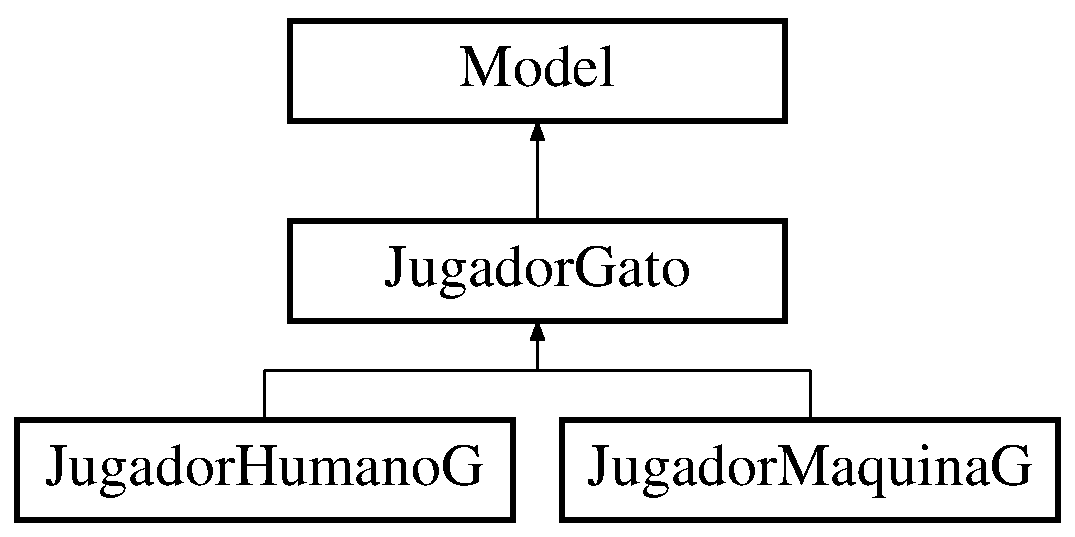
\includegraphics[height=3.000000cm]{class_jugador_gato}
\end{center}
\end{figure}
\subsection*{Public Member Functions}
\begin{DoxyCompactItemize}
\item 
\hyperlink{class_jugador_gato_af067213fcf75bba0584b62224f37aaac}{Jugador\+Gato} (char $\ast$, char, int)
\begin{DoxyCompactList}\small\item\em Constructor. \end{DoxyCompactList}\item 
virtual \hyperlink{class_jugador_gato_aa1ce1ce7e08c10a1411a3fcf70db8927}{$\sim$\+Jugador\+Gato} ()\hypertarget{class_jugador_gato_aa1ce1ce7e08c10a1411a3fcf70db8927}{}\label{class_jugador_gato_aa1ce1ce7e08c10a1411a3fcf70db8927}

\begin{DoxyCompactList}\small\item\em Destructor. \end{DoxyCompactList}\item 
char $\ast$ \hyperlink{class_jugador_gato_a681a58adde0cf273a426d9e628d2cc6a}{get\+Nombre} ()
\begin{DoxyCompactList}\small\item\em Devuelve nombre del jugador. \end{DoxyCompactList}\item 
char \hyperlink{class_jugador_gato_ae62e53c1e01067ab60403f0043c1ac7d}{get\+Caracter} ()
\begin{DoxyCompactList}\small\item\em Devuelve el caracter dle jugador. \end{DoxyCompactList}\item 
int {\bfseries get\+Id} ()\hypertarget{class_jugador_gato_aade24ff7b78d966dacc92576be3cfd32}{}\label{class_jugador_gato_aade24ff7b78d966dacc92576be3cfd32}

\item 
virtual int $\ast$ {\bfseries escoger\+Posicion} ()=0\hypertarget{class_jugador_gato_aeb3128d82c7f772d7cde3742aa8005ce}{}\label{class_jugador_gato_aeb3128d82c7f772d7cde3742aa8005ce}

\item 
void \hyperlink{class_jugador_gato_ade6d9051e9248e0ad50c489966192c1f}{set\+Tablero} (char\mbox{[}3\mbox{]}\mbox{[}3\mbox{]})
\begin{DoxyCompactList}\small\item\em Actualiza el tablero en juego. \end{DoxyCompactList}\end{DoxyCompactItemize}
\subsection*{Protected Attributes}
\begin{DoxyCompactItemize}
\item 
int \hyperlink{class_jugador_gato_a9679414a034dba9d8368f1cd0d0fbc29}{id}
\item 
char $\ast$ \hyperlink{class_jugador_gato_aadcfaa939882268fd6ccfbbeb1573710}{nombre}
\item 
char \hyperlink{class_jugador_gato_a813bdc504edeb75c4fbbea7209e3f6d8}{caracter}
\item 
int $\ast$ \hyperlink{class_jugador_gato_a72bb79fbed6943c62fd54dbb7a8c6ff9}{posicion}
\item 
char \hyperlink{class_jugador_gato_afda277644a559764840c795c936ee22c}{tablero} \mbox{[}3\mbox{]}\mbox{[}3\mbox{]}
\end{DoxyCompactItemize}


\subsection{Detailed Description}
Atributos y metodos de \hyperlink{class_jugador_gato}{Jugador\+Gato}. 

\subsection{Constructor \& Destructor Documentation}
\index{Jugador\+Gato@{Jugador\+Gato}!Jugador\+Gato@{Jugador\+Gato}}
\index{Jugador\+Gato@{Jugador\+Gato}!Jugador\+Gato@{Jugador\+Gato}}
\subsubsection[{\texorpdfstring{Jugador\+Gato(char $\ast$, char, int)}{JugadorGato(char *, char, int)}}]{\setlength{\rightskip}{0pt plus 5cm}Jugador\+Gato\+::\+Jugador\+Gato (
\begin{DoxyParamCaption}
\item[{char $\ast$}]{nombre, }
\item[{char}]{caracter, }
\item[{int}]{id}
\end{DoxyParamCaption}
)}\hypertarget{class_jugador_gato_af067213fcf75bba0584b62224f37aaac}{}\label{class_jugador_gato_af067213fcf75bba0584b62224f37aaac}


Constructor. 


\begin{DoxyParams}{Parameters}
{\em nombre} & char $\ast$ \\
\hline
{\em caracter} & char \\
\hline
\end{DoxyParams}


\subsection{Member Function Documentation}
\index{Jugador\+Gato@{Jugador\+Gato}!get\+Caracter@{get\+Caracter}}
\index{get\+Caracter@{get\+Caracter}!Jugador\+Gato@{Jugador\+Gato}}
\subsubsection[{\texorpdfstring{get\+Caracter()}{getCaracter()}}]{\setlength{\rightskip}{0pt plus 5cm}char Jugador\+Gato\+::get\+Caracter (
\begin{DoxyParamCaption}
{}
\end{DoxyParamCaption}
)}\hypertarget{class_jugador_gato_ae62e53c1e01067ab60403f0043c1ac7d}{}\label{class_jugador_gato_ae62e53c1e01067ab60403f0043c1ac7d}


Devuelve el caracter dle jugador. 

\begin{DoxyReturn}{Returns}
caracter char 
\end{DoxyReturn}
\index{Jugador\+Gato@{Jugador\+Gato}!get\+Nombre@{get\+Nombre}}
\index{get\+Nombre@{get\+Nombre}!Jugador\+Gato@{Jugador\+Gato}}
\subsubsection[{\texorpdfstring{get\+Nombre()}{getNombre()}}]{\setlength{\rightskip}{0pt plus 5cm}char $\ast$ Jugador\+Gato\+::get\+Nombre (
\begin{DoxyParamCaption}
{}
\end{DoxyParamCaption}
)}\hypertarget{class_jugador_gato_a681a58adde0cf273a426d9e628d2cc6a}{}\label{class_jugador_gato_a681a58adde0cf273a426d9e628d2cc6a}


Devuelve nombre del jugador. 

\begin{DoxyReturn}{Returns}
nombre char$\ast$ 
\end{DoxyReturn}
\index{Jugador\+Gato@{Jugador\+Gato}!set\+Tablero@{set\+Tablero}}
\index{set\+Tablero@{set\+Tablero}!Jugador\+Gato@{Jugador\+Gato}}
\subsubsection[{\texorpdfstring{set\+Tablero(char[3][3])}{setTablero(char[3][3])}}]{\setlength{\rightskip}{0pt plus 5cm}void Jugador\+Gato\+::set\+Tablero (
\begin{DoxyParamCaption}
\item[{char}]{table\mbox{[}3\mbox{]}\mbox{[}3\mbox{]}}
\end{DoxyParamCaption}
)}\hypertarget{class_jugador_gato_ade6d9051e9248e0ad50c489966192c1f}{}\label{class_jugador_gato_ade6d9051e9248e0ad50c489966192c1f}


Actualiza el tablero en juego. 


\begin{DoxyParams}{Parameters}
{\em table\mbox{[}3\mbox{]}\mbox{[}3\mbox{]}} & char. Tablero del juego \\
\hline
\end{DoxyParams}


\subsection{Member Data Documentation}
\index{Jugador\+Gato@{Jugador\+Gato}!caracter@{caracter}}
\index{caracter@{caracter}!Jugador\+Gato@{Jugador\+Gato}}
\subsubsection[{\texorpdfstring{caracter}{caracter}}]{\setlength{\rightskip}{0pt plus 5cm}char Jugador\+Gato\+::caracter\hspace{0.3cm}{\ttfamily [protected]}}\hypertarget{class_jugador_gato_a813bdc504edeb75c4fbbea7209e3f6d8}{}\label{class_jugador_gato_a813bdc504edeb75c4fbbea7209e3f6d8}
varible char caracter (X o O) \index{Jugador\+Gato@{Jugador\+Gato}!id@{id}}
\index{id@{id}!Jugador\+Gato@{Jugador\+Gato}}
\subsubsection[{\texorpdfstring{id}{id}}]{\setlength{\rightskip}{0pt plus 5cm}int Jugador\+Gato\+::id\hspace{0.3cm}{\ttfamily [protected]}}\hypertarget{class_jugador_gato_a9679414a034dba9d8368f1cd0d0fbc29}{}\label{class_jugador_gato_a9679414a034dba9d8368f1cd0d0fbc29}
varible integer id. Diferencia a cada jugador PC \index{Jugador\+Gato@{Jugador\+Gato}!nombre@{nombre}}
\index{nombre@{nombre}!Jugador\+Gato@{Jugador\+Gato}}
\subsubsection[{\texorpdfstring{nombre}{nombre}}]{\setlength{\rightskip}{0pt plus 5cm}char$\ast$ Jugador\+Gato\+::nombre\hspace{0.3cm}{\ttfamily [protected]}}\hypertarget{class_jugador_gato_aadcfaa939882268fd6ccfbbeb1573710}{}\label{class_jugador_gato_aadcfaa939882268fd6ccfbbeb1573710}
varible char $\ast$ nombre \index{Jugador\+Gato@{Jugador\+Gato}!posicion@{posicion}}
\index{posicion@{posicion}!Jugador\+Gato@{Jugador\+Gato}}
\subsubsection[{\texorpdfstring{posicion}{posicion}}]{\setlength{\rightskip}{0pt plus 5cm}int$\ast$ Jugador\+Gato\+::posicion\hspace{0.3cm}{\ttfamily [protected]}}\hypertarget{class_jugador_gato_a72bb79fbed6943c62fd54dbb7a8c6ff9}{}\label{class_jugador_gato_a72bb79fbed6943c62fd54dbb7a8c6ff9}
varible integer $\ast$ posicion. Donde se ingresara el caracter. \index{Jugador\+Gato@{Jugador\+Gato}!tablero@{tablero}}
\index{tablero@{tablero}!Jugador\+Gato@{Jugador\+Gato}}
\subsubsection[{\texorpdfstring{tablero}{tablero}}]{\setlength{\rightskip}{0pt plus 5cm}char Jugador\+Gato\+::tablero\mbox{[}3\mbox{]}\mbox{[}3\mbox{]}\hspace{0.3cm}{\ttfamily [protected]}}\hypertarget{class_jugador_gato_afda277644a559764840c795c936ee22c}{}\label{class_jugador_gato_afda277644a559764840c795c936ee22c}
varible char tablero. Tablero con el que se esta jugando 

The documentation for this class was generated from the following files\+:\begin{DoxyCompactItemize}
\item 
C\+:/\+Users/\+Alexa Duarte/\+Desktop/\+Examen\+I-\/\+Juegos\+Y\+Jugadores\+Polimorficos/\+Examen\+I-\/\+Juegos\+Y\+Jugadores\+Polimorficos/Jugador\+Gato.\+h\item 
C\+:/\+Users/\+Alexa Duarte/\+Desktop/\+Examen\+I-\/\+Juegos\+Y\+Jugadores\+Polimorficos/\+Examen\+I-\/\+Juegos\+Y\+Jugadores\+Polimorficos/Jugador\+Gato.\+cpp\end{DoxyCompactItemize}

\hypertarget{class_jugador_humano}{}\section{Jugador\+Humano Class Reference}
\label{class_jugador_humano}\index{Jugador\+Humano@{Jugador\+Humano}}


Metodos del jugador humano. Hija de \hyperlink{class_jugador21}{Jugador21}.  




{\ttfamily \#include $<$Jugador\+Humano.\+h$>$}

Inheritance diagram for Jugador\+Humano\+:\begin{figure}[H]
\begin{center}
\leavevmode
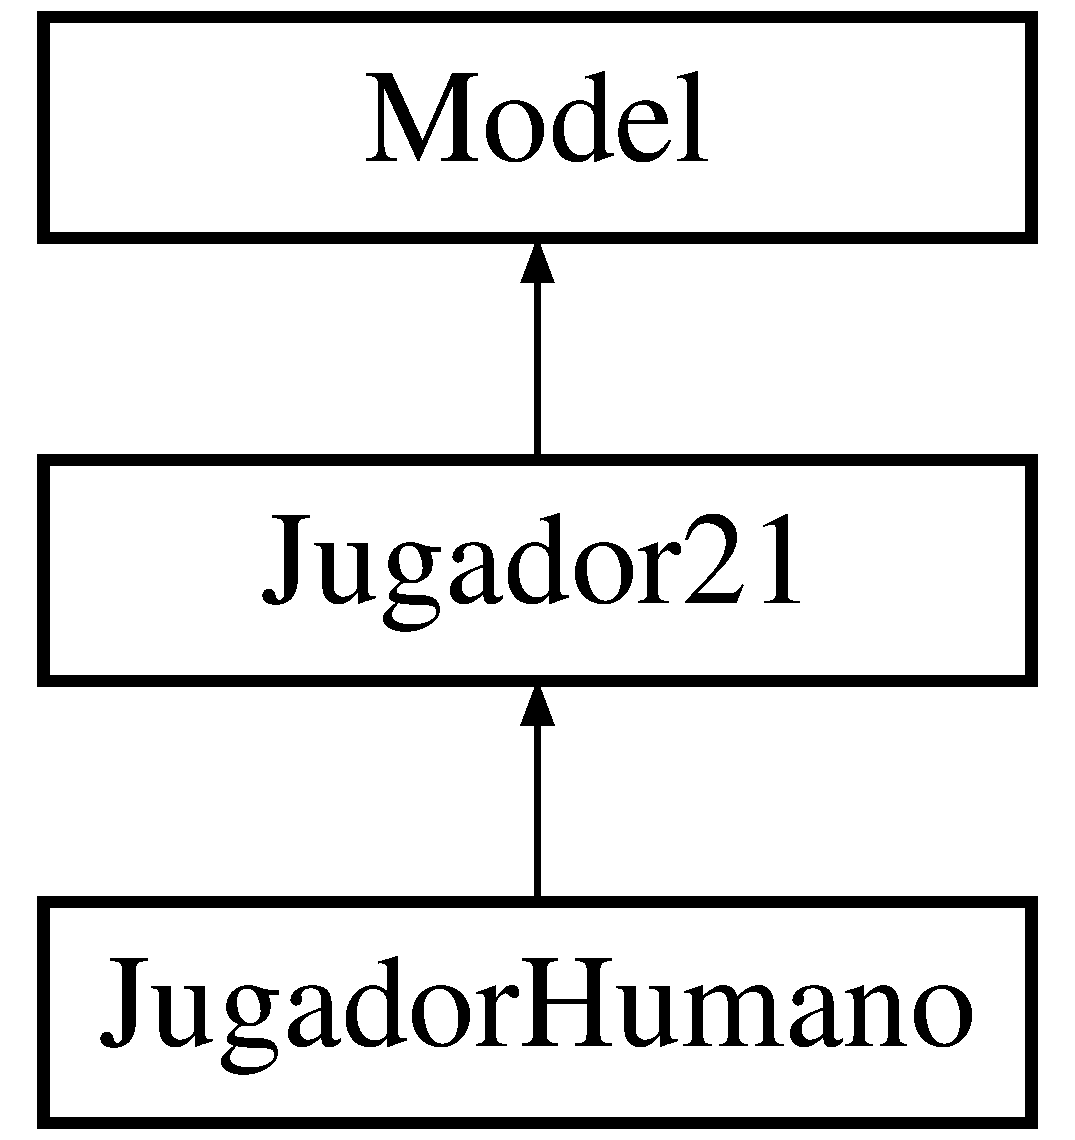
\includegraphics[height=3.000000cm]{class_jugador_humano}
\end{center}
\end{figure}
\subsection*{Public Member Functions}
\begin{DoxyCompactItemize}
\item 
\hyperlink{class_jugador_humano_add1814239a072772aa1e8720b2dc69da}{Jugador\+Humano} (char $\ast$, int)
\begin{DoxyCompactList}\small\item\em Constructor. \end{DoxyCompactList}\item 
virtual \hyperlink{class_jugador_humano_a6da9f2a6ff013128e1ceb75e0e871620}{$\sim$\+Jugador\+Humano} ()\hypertarget{class_jugador_humano_a6da9f2a6ff013128e1ceb75e0e871620}{}\label{class_jugador_humano_a6da9f2a6ff013128e1ceb75e0e871620}

\begin{DoxyCompactList}\small\item\em Destructor. \end{DoxyCompactList}\end{DoxyCompactItemize}
\subsection*{Additional Inherited Members}


\subsection{Detailed Description}
Metodos del jugador humano. Hija de \hyperlink{class_jugador21}{Jugador21}. 

\subsection{Constructor \& Destructor Documentation}
\index{Jugador\+Humano@{Jugador\+Humano}!Jugador\+Humano@{Jugador\+Humano}}
\index{Jugador\+Humano@{Jugador\+Humano}!Jugador\+Humano@{Jugador\+Humano}}
\subsubsection[{\texorpdfstring{Jugador\+Humano(char $\ast$, int)}{JugadorHumano(char *, int)}}]{\setlength{\rightskip}{0pt plus 5cm}Jugador\+Humano\+::\+Jugador\+Humano (
\begin{DoxyParamCaption}
\item[{char $\ast$}]{nombre, }
\item[{int}]{numero\+Jugador}
\end{DoxyParamCaption}
)}\hypertarget{class_jugador_humano_add1814239a072772aa1e8720b2dc69da}{}\label{class_jugador_humano_add1814239a072772aa1e8720b2dc69da}


Constructor. 


\begin{DoxyParams}{Parameters}
{\em nombre} & char $\ast$ \\
\hline
{\em numero\+Jugador} & int \\
\hline
\end{DoxyParams}


The documentation for this class was generated from the following files\+:\begin{DoxyCompactItemize}
\item 
C\+:/\+Users/\+Alexa Duarte/\+Desktop/\+Examen\+I-\/\+Juegos\+Y\+Jugadores\+Polimorficos/\+Examen\+I-\/\+Juegos\+Y\+Jugadores\+Polimorficos/Jugador\+Humano.\+h\item 
C\+:/\+Users/\+Alexa Duarte/\+Desktop/\+Examen\+I-\/\+Juegos\+Y\+Jugadores\+Polimorficos/\+Examen\+I-\/\+Juegos\+Y\+Jugadores\+Polimorficos/Jugador\+Humano.\+cpp\end{DoxyCompactItemize}

\hypertarget{class_jugador_humano_g}{}\section{Jugador\+HumanoG Class Reference}
\label{class_jugador_humano_g}\index{Jugador\+HumanoG@{Jugador\+HumanoG}}


Metodos del \hyperlink{class_jugador_humano_g}{Jugador\+HumanoG}. Hija de \hyperlink{class_jugador_gato}{Jugador\+Gato}.  




{\ttfamily \#include $<$Jugador\+Humano\+G.\+h$>$}

Inheritance diagram for Jugador\+HumanoG\+:\begin{figure}[H]
\begin{center}
\leavevmode
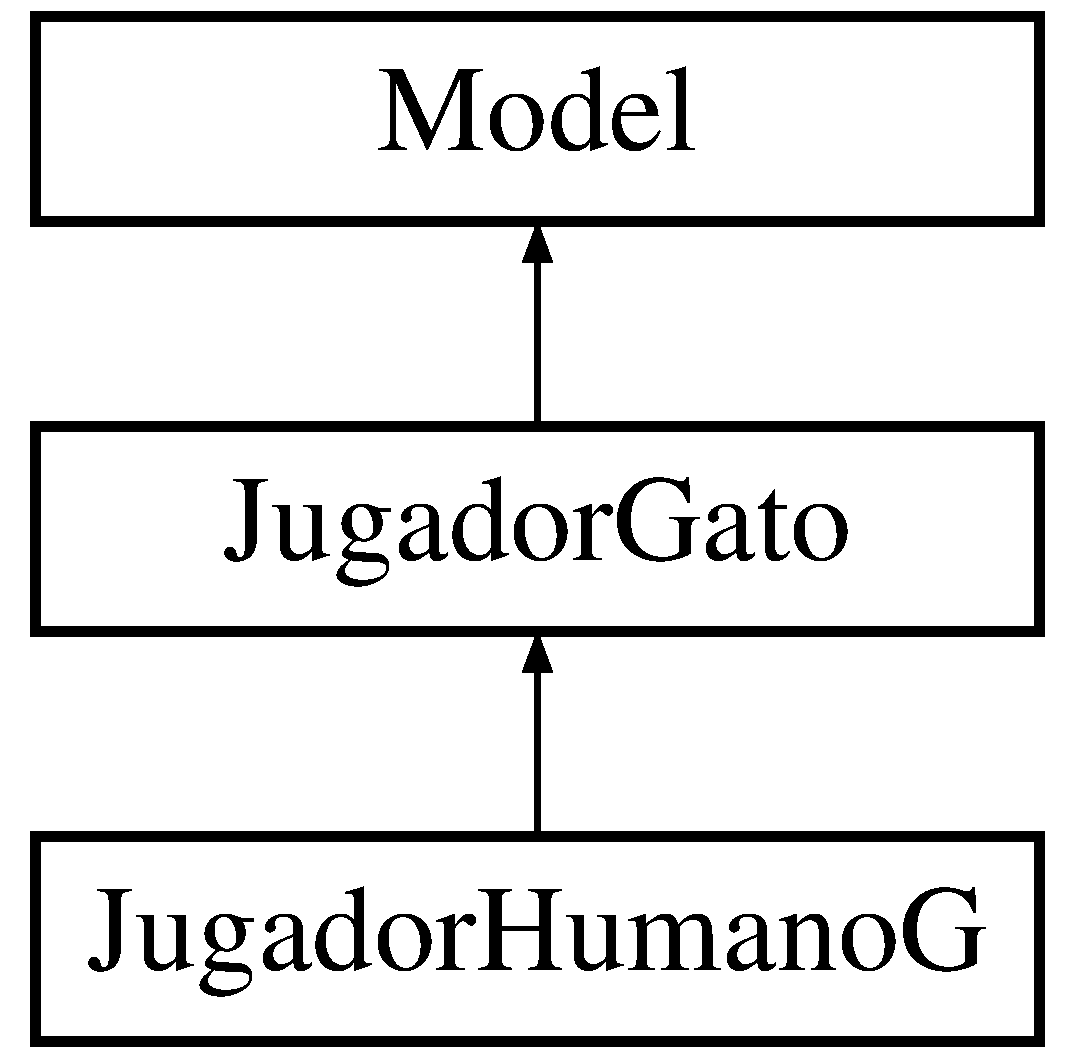
\includegraphics[height=3.000000cm]{class_jugador_humano_g}
\end{center}
\end{figure}
\subsection*{Public Member Functions}
\begin{DoxyCompactItemize}
\item 
\hyperlink{class_jugador_humano_g_a83d1be7d6e1365740c5d3aaf2083882d}{Jugador\+HumanoG} (char $\ast$, char, int)
\begin{DoxyCompactList}\small\item\em Constructor. \end{DoxyCompactList}\item 
virtual \hyperlink{class_jugador_humano_g_abf6b59a6720c3797cca328f49b06bf14}{$\sim$\+Jugador\+HumanoG} ()\hypertarget{class_jugador_humano_g_abf6b59a6720c3797cca328f49b06bf14}{}\label{class_jugador_humano_g_abf6b59a6720c3797cca328f49b06bf14}

\begin{DoxyCompactList}\small\item\em Destructor. \end{DoxyCompactList}\end{DoxyCompactItemize}
\subsection*{Additional Inherited Members}


\subsection{Detailed Description}
Metodos del \hyperlink{class_jugador_humano_g}{Jugador\+HumanoG}. Hija de \hyperlink{class_jugador_gato}{Jugador\+Gato}. 

\subsection{Constructor \& Destructor Documentation}
\index{Jugador\+HumanoG@{Jugador\+HumanoG}!Jugador\+HumanoG@{Jugador\+HumanoG}}
\index{Jugador\+HumanoG@{Jugador\+HumanoG}!Jugador\+HumanoG@{Jugador\+HumanoG}}
\subsubsection[{\texorpdfstring{Jugador\+Humano\+G(char $\ast$, char, int)}{JugadorHumanoG(char *, char, int)}}]{\setlength{\rightskip}{0pt plus 5cm}Jugador\+Humano\+G\+::\+Jugador\+HumanoG (
\begin{DoxyParamCaption}
\item[{char $\ast$}]{nombre, }
\item[{char}]{caracter, }
\item[{int}]{id}
\end{DoxyParamCaption}
)}\hypertarget{class_jugador_humano_g_a83d1be7d6e1365740c5d3aaf2083882d}{}\label{class_jugador_humano_g_a83d1be7d6e1365740c5d3aaf2083882d}


Constructor. 


\begin{DoxyParams}{Parameters}
{\em nombre} & char $\ast$ \\
\hline
{\em caracter} & char \\
\hline
\end{DoxyParams}


The documentation for this class was generated from the following files\+:\begin{DoxyCompactItemize}
\item 
C\+:/\+Users/\+Alexa Duarte/\+Desktop/\+Examen\+I-\/\+Juegos\+Y\+Jugadores\+Polimorficos/\+Examen\+I-\/\+Juegos\+Y\+Jugadores\+Polimorficos/Jugador\+Humano\+G.\+h\item 
C\+:/\+Users/\+Alexa Duarte/\+Desktop/\+Examen\+I-\/\+Juegos\+Y\+Jugadores\+Polimorficos/\+Examen\+I-\/\+Juegos\+Y\+Jugadores\+Polimorficos/Jugador\+Humano\+G.\+cpp\end{DoxyCompactItemize}

\hypertarget{class_jugador_maquina}{}\section{Jugador\+Maquina Class Reference}
\label{class_jugador_maquina}\index{Jugador\+Maquina@{Jugador\+Maquina}}


Metodos de \hyperlink{class_jugador_maquina}{Jugador\+Maquina}. Hija de \hyperlink{class_jugador21}{Jugador21}.  




{\ttfamily \#include $<$Jugador\+Maquina.\+h$>$}

Inheritance diagram for Jugador\+Maquina\+:\begin{figure}[H]
\begin{center}
\leavevmode
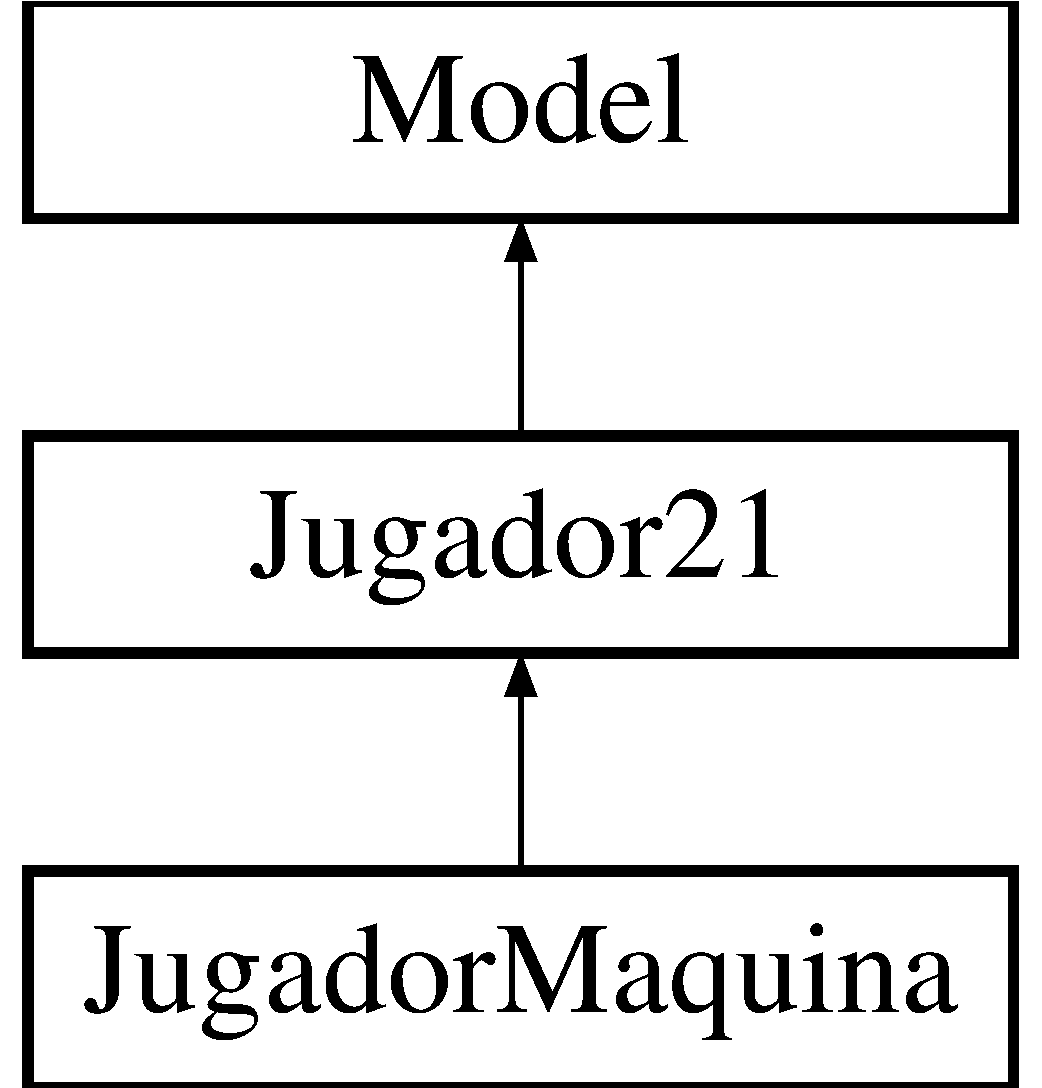
\includegraphics[height=3.000000cm]{class_jugador_maquina}
\end{center}
\end{figure}
\subsection*{Public Member Functions}
\begin{DoxyCompactItemize}
\item 
\hyperlink{class_jugador_maquina_ac67d579c7aa41ca6ecdfd424f5d8001d}{Jugador\+Maquina} (char $\ast$, int)
\begin{DoxyCompactList}\small\item\em Constructor. \end{DoxyCompactList}\item 
virtual \hyperlink{class_jugador_maquina_a0d360dbd742297fd73ffcdc0d028abe5}{$\sim$\+Jugador\+Maquina} ()\hypertarget{class_jugador_maquina_a0d360dbd742297fd73ffcdc0d028abe5}{}\label{class_jugador_maquina_a0d360dbd742297fd73ffcdc0d028abe5}

\begin{DoxyCompactList}\small\item\em Destructor. \end{DoxyCompactList}\end{DoxyCompactItemize}
\subsection*{Additional Inherited Members}


\subsection{Detailed Description}
Metodos de \hyperlink{class_jugador_maquina}{Jugador\+Maquina}. Hija de \hyperlink{class_jugador21}{Jugador21}. 

\subsection{Constructor \& Destructor Documentation}
\index{Jugador\+Maquina@{Jugador\+Maquina}!Jugador\+Maquina@{Jugador\+Maquina}}
\index{Jugador\+Maquina@{Jugador\+Maquina}!Jugador\+Maquina@{Jugador\+Maquina}}
\subsubsection[{\texorpdfstring{Jugador\+Maquina(char $\ast$, int)}{JugadorMaquina(char *, int)}}]{\setlength{\rightskip}{0pt plus 5cm}Jugador\+Maquina\+::\+Jugador\+Maquina (
\begin{DoxyParamCaption}
\item[{char $\ast$}]{nombre, }
\item[{int}]{numero\+Jugador}
\end{DoxyParamCaption}
)}\hypertarget{class_jugador_maquina_ac67d579c7aa41ca6ecdfd424f5d8001d}{}\label{class_jugador_maquina_ac67d579c7aa41ca6ecdfd424f5d8001d}


Constructor. 


\begin{DoxyParams}{Parameters}
{\em nombre} & char $\ast$ \\
\hline
{\em numero\+Jugador} & int \\
\hline
\end{DoxyParams}


The documentation for this class was generated from the following files\+:\begin{DoxyCompactItemize}
\item 
C\+:/\+Users/\+Alexa Duarte/\+Desktop/\+Examen\+I-\/\+Juegos\+Y\+Jugadores\+Polimorficos/\+Examen\+I-\/\+Juegos\+Y\+Jugadores\+Polimorficos/Jugador\+Maquina.\+h\item 
C\+:/\+Users/\+Alexa Duarte/\+Desktop/\+Examen\+I-\/\+Juegos\+Y\+Jugadores\+Polimorficos/\+Examen\+I-\/\+Juegos\+Y\+Jugadores\+Polimorficos/Jugador\+Maquina.\+cpp\end{DoxyCompactItemize}

\hypertarget{class_jugador_maquina_g}{}\section{Jugador\+MaquinaG Class Reference}
\label{class_jugador_maquina_g}\index{Jugador\+MaquinaG@{Jugador\+MaquinaG}}


Atributos y metodos de \hyperlink{class_jugador_maquina_g}{Jugador\+MaquinaG}. Hija de \hyperlink{class_jugador_gato}{Jugador\+Gato}.  




{\ttfamily \#include $<$Jugador\+Maquina\+G.\+h$>$}

Inheritance diagram for Jugador\+MaquinaG\+:\begin{figure}[H]
\begin{center}
\leavevmode
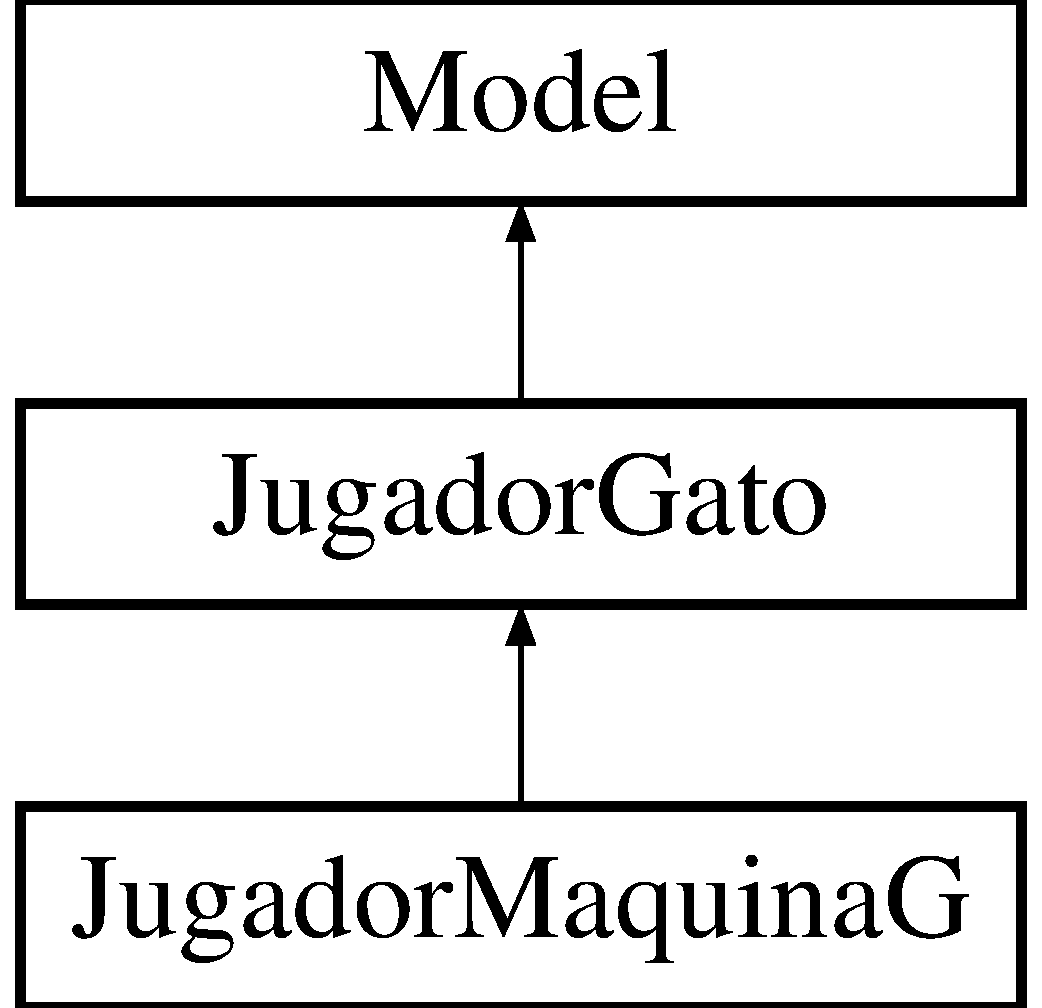
\includegraphics[height=3.000000cm]{class_jugador_maquina_g}
\end{center}
\end{figure}
\subsection*{Public Member Functions}
\begin{DoxyCompactItemize}
\item 
\hyperlink{class_jugador_maquina_g_aa76e12483ff12147f0adce95c9c6143f}{Jugador\+MaquinaG} (char, int)
\begin{DoxyCompactList}\small\item\em Constructor. \end{DoxyCompactList}\item 
virtual \hyperlink{class_jugador_maquina_g_ae60c6b2bfb8397cf05af73326bf7fa8f}{$\sim$\+Jugador\+MaquinaG} ()\hypertarget{class_jugador_maquina_g_ae60c6b2bfb8397cf05af73326bf7fa8f}{}\label{class_jugador_maquina_g_ae60c6b2bfb8397cf05af73326bf7fa8f}

\begin{DoxyCompactList}\small\item\em Destructor. \end{DoxyCompactList}\end{DoxyCompactItemize}
\subsection*{Additional Inherited Members}


\subsection{Detailed Description}
Atributos y metodos de \hyperlink{class_jugador_maquina_g}{Jugador\+MaquinaG}. Hija de \hyperlink{class_jugador_gato}{Jugador\+Gato}. 

\subsection{Constructor \& Destructor Documentation}
\index{Jugador\+MaquinaG@{Jugador\+MaquinaG}!Jugador\+MaquinaG@{Jugador\+MaquinaG}}
\index{Jugador\+MaquinaG@{Jugador\+MaquinaG}!Jugador\+MaquinaG@{Jugador\+MaquinaG}}
\subsubsection[{\texorpdfstring{Jugador\+Maquina\+G(char, int)}{JugadorMaquinaG(char, int)}}]{\setlength{\rightskip}{0pt plus 5cm}Jugador\+Maquina\+G\+::\+Jugador\+MaquinaG (
\begin{DoxyParamCaption}
\item[{char}]{caracter, }
\item[{int}]{id}
\end{DoxyParamCaption}
)}\hypertarget{class_jugador_maquina_g_aa76e12483ff12147f0adce95c9c6143f}{}\label{class_jugador_maquina_g_aa76e12483ff12147f0adce95c9c6143f}


Constructor. 


\begin{DoxyParams}{Parameters}
{\em caracter} & char \\
\hline
\end{DoxyParams}


The documentation for this class was generated from the following files\+:\begin{DoxyCompactItemize}
\item 
C\+:/\+Users/\+Alexa Duarte/\+Desktop/\+Examen\+I-\/\+Juegos\+Y\+Jugadores\+Polimorficos/\+Examen\+I-\/\+Juegos\+Y\+Jugadores\+Polimorficos/Jugador\+Maquina\+G.\+h\item 
C\+:/\+Users/\+Alexa Duarte/\+Desktop/\+Examen\+I-\/\+Juegos\+Y\+Jugadores\+Polimorficos/\+Examen\+I-\/\+Juegos\+Y\+Jugadores\+Polimorficos/Jugador\+Maquina\+G.\+cpp\end{DoxyCompactItemize}

\hypertarget{class_model}{}\section{Model Class Reference}
\label{class_model}\index{Model@{Model}}


Modelo de las clases.  




{\ttfamily \#include $<$Model.\+h$>$}

Inheritance diagram for Model\+:\begin{figure}[H]
\begin{center}
\leavevmode
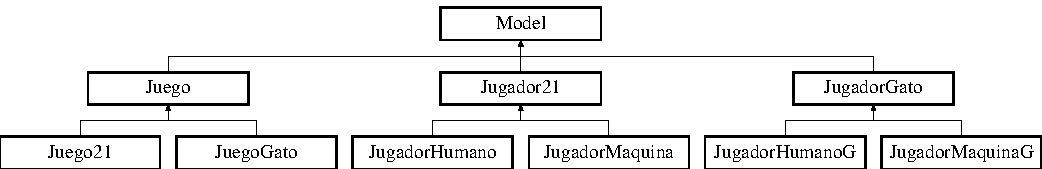
\includegraphics[height=2.258065cm]{class_model}
\end{center}
\end{figure}
\subsection*{Public Member Functions}
\begin{DoxyCompactItemize}
\item 
\hyperlink{class_model_ae3b375de5f6df4faf74a95d64748e048}{Model} ()\hypertarget{class_model_ae3b375de5f6df4faf74a95d64748e048}{}\label{class_model_ae3b375de5f6df4faf74a95d64748e048}

\begin{DoxyCompactList}\small\item\em Constructor. \end{DoxyCompactList}\item 
virtual \hyperlink{class_model_ad6ebd2062a0b823db841a0b88baac4c0}{$\sim$\+Model} ()\hypertarget{class_model_ad6ebd2062a0b823db841a0b88baac4c0}{}\label{class_model_ad6ebd2062a0b823db841a0b88baac4c0}

\begin{DoxyCompactList}\small\item\em Destructor. \end{DoxyCompactList}\item 
void \hyperlink{class_model_a5cdcdd24e529d6a8c8e0804d41e1c1fc}{add\+View} (\hyperlink{class_view}{View} $\ast$)
\begin{DoxyCompactList}\small\item\em Agrega vistas a la lista de vistas. \end{DoxyCompactList}\item 
void \hyperlink{class_model_a9bfb8dc6d332b86592b08050ca0debda}{delete\+View} (\hyperlink{class_view}{View} $\ast$)
\begin{DoxyCompactList}\small\item\em Elimina vistas de la lista de vistas. \end{DoxyCompactList}\item 
void \hyperlink{class_model_a9bb776b622153d782936d55e80dbb8c6}{notify\+Output} (char $\ast$)
\begin{DoxyCompactList}\small\item\em Notifica de output tipo char $\ast$. \end{DoxyCompactList}\item 
void \hyperlink{class_model_a5ab8965d490fee7f941a061c510eba08}{notify\+Output\+Int} (int)
\begin{DoxyCompactList}\small\item\em Notifica de output tipo int. \end{DoxyCompactList}\item 
void \hyperlink{class_model_a2428b409ff14fbd7247465850481f822}{notify\+Output\+Char} (char)
\begin{DoxyCompactList}\small\item\em Notifica de un output tipo char. \end{DoxyCompactList}\item 
char $\ast$ \hyperlink{class_model_ae1a72659a294ad394d7bad30c1a7d9c4}{notify\+Input} (char $\ast$)
\begin{DoxyCompactList}\small\item\em Notifica de un input tipo char $\ast$. \end{DoxyCompactList}\item 
int \hyperlink{class_model_a6363623b712b863ac40ba6bd1ab187df}{notify\+Input\+Int} (char $\ast$)
\begin{DoxyCompactList}\small\item\em Notifica de un input tipo int. \end{DoxyCompactList}\item 
char \hyperlink{class_model_a7db0b973c915d48c7def55b24797e782}{notify\+Input\+Char} (char $\ast$)
\begin{DoxyCompactList}\small\item\em Notifica de un input tipo char. \end{DoxyCompactList}\item 
list$<$ \hyperlink{class_view}{View} $\ast$ $>$ \hyperlink{class_model_a8b482b2e574b1102572c96052b6ece17}{get\+List} ()
\begin{DoxyCompactList}\small\item\em Devuelve la lista de vistas. \end{DoxyCompactList}\end{DoxyCompactItemize}
\subsection*{Protected Attributes}
\begin{DoxyCompactItemize}
\item 
list$<$ \hyperlink{class_view}{View} $\ast$ $>$ {\bfseries views}\hypertarget{class_model_a4bf8f660ee7b53d0c5b00cb7b605a9f0}{}\label{class_model_a4bf8f660ee7b53d0c5b00cb7b605a9f0}

\end{DoxyCompactItemize}


\subsection{Detailed Description}
Modelo de las clases. 

\subsection{Member Function Documentation}
\index{Model@{Model}!add\+View@{add\+View}}
\index{add\+View@{add\+View}!Model@{Model}}
\subsubsection[{\texorpdfstring{add\+View(\+View $\ast$)}{addView(View *)}}]{\setlength{\rightskip}{0pt plus 5cm}void Model\+::add\+View (
\begin{DoxyParamCaption}
\item[{{\bf View} $\ast$}]{vista}
\end{DoxyParamCaption}
)}\hypertarget{class_model_a5cdcdd24e529d6a8c8e0804d41e1c1fc}{}\label{class_model_a5cdcdd24e529d6a8c8e0804d41e1c1fc}


Agrega vistas a la lista de vistas. 


\begin{DoxyParams}{Parameters}
{\em $\ast$} & vista \hyperlink{class_view}{View}. Lista a agregar. \\
\hline
\end{DoxyParams}
\index{Model@{Model}!delete\+View@{delete\+View}}
\index{delete\+View@{delete\+View}!Model@{Model}}
\subsubsection[{\texorpdfstring{delete\+View(\+View $\ast$)}{deleteView(View *)}}]{\setlength{\rightskip}{0pt plus 5cm}void Model\+::delete\+View (
\begin{DoxyParamCaption}
\item[{{\bf View} $\ast$}]{vista}
\end{DoxyParamCaption}
)}\hypertarget{class_model_a9bfb8dc6d332b86592b08050ca0debda}{}\label{class_model_a9bfb8dc6d332b86592b08050ca0debda}


Elimina vistas de la lista de vistas. 


\begin{DoxyParams}{Parameters}
{\em vista} & \hyperlink{class_view}{View} $\ast$. Lista a eliminar. \\
\hline
\end{DoxyParams}
\index{Model@{Model}!get\+List@{get\+List}}
\index{get\+List@{get\+List}!Model@{Model}}
\subsubsection[{\texorpdfstring{get\+List()}{getList()}}]{\setlength{\rightskip}{0pt plus 5cm}list$<$ {\bf View} $\ast$ $>$ Model\+::get\+List (
\begin{DoxyParamCaption}
{}
\end{DoxyParamCaption}
)}\hypertarget{class_model_a8b482b2e574b1102572c96052b6ece17}{}\label{class_model_a8b482b2e574b1102572c96052b6ece17}


Devuelve la lista de vistas. 

\begin{DoxyReturn}{Returns}
list$<$\+View$\ast$$>$. Listas de vistas. 
\end{DoxyReturn}
\index{Model@{Model}!notify\+Input@{notify\+Input}}
\index{notify\+Input@{notify\+Input}!Model@{Model}}
\subsubsection[{\texorpdfstring{notify\+Input(char $\ast$)}{notifyInput(char *)}}]{\setlength{\rightskip}{0pt plus 5cm}char $\ast$ Model\+::notify\+Input (
\begin{DoxyParamCaption}
\item[{char $\ast$}]{msj}
\end{DoxyParamCaption}
)}\hypertarget{class_model_ae1a72659a294ad394d7bad30c1a7d9c4}{}\label{class_model_ae1a72659a294ad394d7bad30c1a7d9c4}


Notifica de un input tipo char $\ast$. 


\begin{DoxyParams}{Parameters}
{\em msj} & char $\ast$. Mensaje a mostrar. \\
\hline
\end{DoxyParams}
\begin{DoxyReturn}{Returns}
char $\ast$ mensaje introducido 
\end{DoxyReturn}
\index{Model@{Model}!notify\+Input\+Char@{notify\+Input\+Char}}
\index{notify\+Input\+Char@{notify\+Input\+Char}!Model@{Model}}
\subsubsection[{\texorpdfstring{notify\+Input\+Char(char $\ast$)}{notifyInputChar(char *)}}]{\setlength{\rightskip}{0pt plus 5cm}char Model\+::notify\+Input\+Char (
\begin{DoxyParamCaption}
\item[{char $\ast$}]{msj}
\end{DoxyParamCaption}
)}\hypertarget{class_model_a7db0b973c915d48c7def55b24797e782}{}\label{class_model_a7db0b973c915d48c7def55b24797e782}


Notifica de un input tipo char. 


\begin{DoxyParams}{Parameters}
{\em msj} & char $\ast$. Mensaje a mostrar. \\
\hline
\end{DoxyParams}
\begin{DoxyReturn}{Returns}
char. Caracter introducido. 
\end{DoxyReturn}
\index{Model@{Model}!notify\+Input\+Int@{notify\+Input\+Int}}
\index{notify\+Input\+Int@{notify\+Input\+Int}!Model@{Model}}
\subsubsection[{\texorpdfstring{notify\+Input\+Int(char $\ast$)}{notifyInputInt(char *)}}]{\setlength{\rightskip}{0pt plus 5cm}int Model\+::notify\+Input\+Int (
\begin{DoxyParamCaption}
\item[{char $\ast$}]{msj}
\end{DoxyParamCaption}
)}\hypertarget{class_model_a6363623b712b863ac40ba6bd1ab187df}{}\label{class_model_a6363623b712b863ac40ba6bd1ab187df}


Notifica de un input tipo int. 


\begin{DoxyParams}{Parameters}
{\em msj} & char $\ast$. Mensaje a mostrar. \\
\hline
\end{DoxyParams}
\begin{DoxyReturn}{Returns}
int. Numero introducido. 
\end{DoxyReturn}
\index{Model@{Model}!notify\+Output@{notify\+Output}}
\index{notify\+Output@{notify\+Output}!Model@{Model}}
\subsubsection[{\texorpdfstring{notify\+Output(char $\ast$)}{notifyOutput(char *)}}]{\setlength{\rightskip}{0pt plus 5cm}void Model\+::notify\+Output (
\begin{DoxyParamCaption}
\item[{char $\ast$}]{msj}
\end{DoxyParamCaption}
)}\hypertarget{class_model_a9bb776b622153d782936d55e80dbb8c6}{}\label{class_model_a9bb776b622153d782936d55e80dbb8c6}


Notifica de output tipo char $\ast$. 


\begin{DoxyParams}{Parameters}
{\em msj} & char $\ast$. Mensaje a mostrar. \\
\hline
\end{DoxyParams}
\index{Model@{Model}!notify\+Output\+Char@{notify\+Output\+Char}}
\index{notify\+Output\+Char@{notify\+Output\+Char}!Model@{Model}}
\subsubsection[{\texorpdfstring{notify\+Output\+Char(char)}{notifyOutputChar(char)}}]{\setlength{\rightskip}{0pt plus 5cm}void Model\+::notify\+Output\+Char (
\begin{DoxyParamCaption}
\item[{char}]{c}
\end{DoxyParamCaption}
)}\hypertarget{class_model_a2428b409ff14fbd7247465850481f822}{}\label{class_model_a2428b409ff14fbd7247465850481f822}


Notifica de un output tipo char. 


\begin{DoxyParams}{Parameters}
{\em c} & char. Caracter a mostrar. \\
\hline
\end{DoxyParams}
\index{Model@{Model}!notify\+Output\+Int@{notify\+Output\+Int}}
\index{notify\+Output\+Int@{notify\+Output\+Int}!Model@{Model}}
\subsubsection[{\texorpdfstring{notify\+Output\+Int(int)}{notifyOutputInt(int)}}]{\setlength{\rightskip}{0pt plus 5cm}void Model\+::notify\+Output\+Int (
\begin{DoxyParamCaption}
\item[{int}]{i}
\end{DoxyParamCaption}
)}\hypertarget{class_model_a5ab8965d490fee7f941a061c510eba08}{}\label{class_model_a5ab8965d490fee7f941a061c510eba08}


Notifica de output tipo int. 


\begin{DoxyParams}{Parameters}
{\em i} & int. Entero a mostrar. \\
\hline
\end{DoxyParams}


The documentation for this class was generated from the following files\+:\begin{DoxyCompactItemize}
\item 
C\+:/\+Users/\+Alexa Duarte/\+Desktop/\+Examen\+I-\/\+Juegos\+Y\+Jugadores\+Polimorficos/\+Examen\+I-\/\+Juegos\+Y\+Jugadores\+Polimorficos/Model.\+h\item 
C\+:/\+Users/\+Alexa Duarte/\+Desktop/\+Examen\+I-\/\+Juegos\+Y\+Jugadores\+Polimorficos/\+Examen\+I-\/\+Juegos\+Y\+Jugadores\+Polimorficos/Model.\+cpp\end{DoxyCompactItemize}

\hypertarget{class_view}{}\section{View Class Reference}
\label{class_view}\index{View@{View}}


Encargada de la vista de las clases.  




{\ttfamily \#include $<$View.\+h$>$}

Inheritance diagram for View\+:\begin{figure}[H]
\begin{center}
\leavevmode
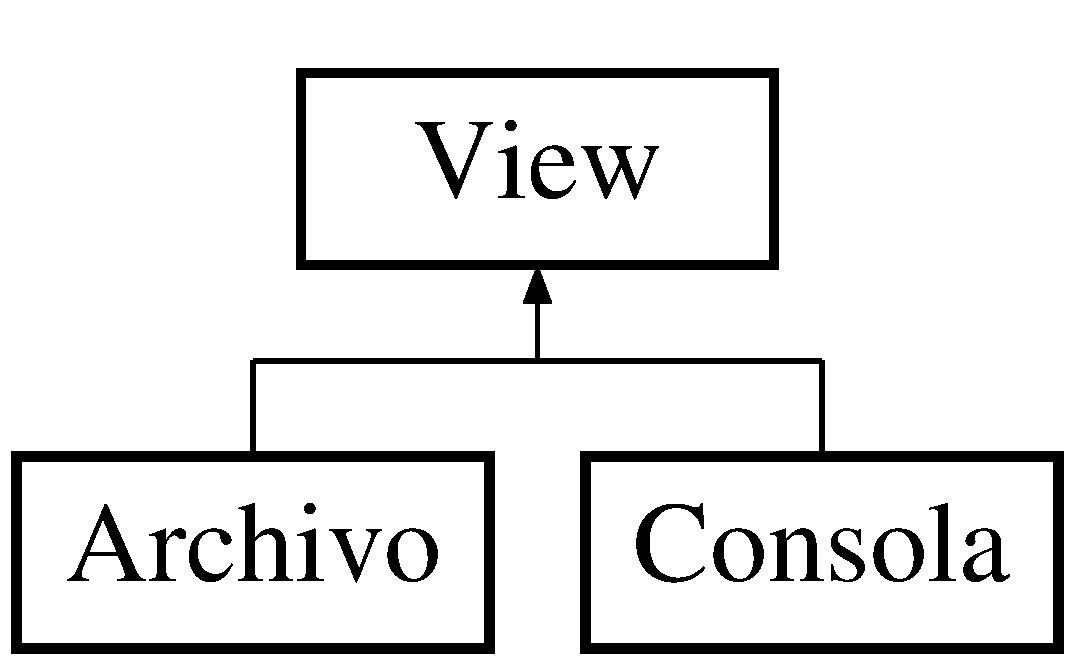
\includegraphics[height=2.000000cm]{class_view}
\end{center}
\end{figure}
\subsection*{Public Member Functions}
\begin{DoxyCompactItemize}
\item 
virtual void {\bfseries output} (char $\ast$)=0\hypertarget{class_view_ab8a6c58a49ba70ecca1677fdaa840b39}{}\label{class_view_ab8a6c58a49ba70ecca1677fdaa840b39}

\item 
virtual void {\bfseries output\+Int} (int)=0\hypertarget{class_view_aa02cebb4b67e05cbf3d7cf30c3ecbb3e}{}\label{class_view_aa02cebb4b67e05cbf3d7cf30c3ecbb3e}

\item 
virtual void {\bfseries output\+Char} (char)=0\hypertarget{class_view_a944f40363167dfccda0408b462fe7593}{}\label{class_view_a944f40363167dfccda0408b462fe7593}

\item 
virtual char $\ast$ {\bfseries input} (char $\ast$)=0\hypertarget{class_view_adcfa16ba54323c94242f60d35c58613c}{}\label{class_view_adcfa16ba54323c94242f60d35c58613c}

\item 
virtual int {\bfseries input\+Int} (char $\ast$)=0\hypertarget{class_view_ae9e0b58ebd710046411e09eae8bc8224}{}\label{class_view_ae9e0b58ebd710046411e09eae8bc8224}

\item 
virtual char {\bfseries input\+Char} (char $\ast$)=0\hypertarget{class_view_aac8eb1e5438a50dcb8334c6805ced205}{}\label{class_view_aac8eb1e5438a50dcb8334c6805ced205}

\end{DoxyCompactItemize}


\subsection{Detailed Description}
Encargada de la vista de las clases. 

The documentation for this class was generated from the following files\+:\begin{DoxyCompactItemize}
\item 
C\+:/\+Users/\+Alexa Duarte/\+Desktop/\+Examen\+I-\/\+Juegos\+Y\+Jugadores\+Polimorficos/\+Examen\+I-\/\+Juegos\+Y\+Jugadores\+Polimorficos/View.\+h\item 
C\+:/\+Users/\+Alexa Duarte/\+Desktop/\+Examen\+I-\/\+Juegos\+Y\+Jugadores\+Polimorficos/\+Examen\+I-\/\+Juegos\+Y\+Jugadores\+Polimorficos/View.\+cpp\end{DoxyCompactItemize}

%--- End generated contents ---

% Index
\backmatter
\newpage
\phantomsection
\clearemptydoublepage
\addcontentsline{toc}{chapter}{Index}
\printindex

\end{document}
